\documentclass[11pt,a4paper]{ctexart}

\usepackage[margin=2.5cm]{geometry}
\usepackage{amsmath,amssymb}
\usepackage{array}
\usepackage{booktabs}
\usepackage{float}
\usepackage{graphicx}
\usepackage{hyperref}
\usepackage{longtable}
\usepackage{tabularx}
\usepackage{xcolor}

\hypersetup{
  colorlinks=true,
  linkcolor=blue!45!black,
  urlcolor=blue!55!black
}

\graphicspath{
  {assets/instruments-report/}
  {assets/games-report/}
  {../baseline/table/assets/}
}

\newcolumntype{Y}{>{\raggedright\arraybackslash}X}
\setlength{\LTleft}{0pt}
\setlength{\LTright}{0pt}

\title{GenRec Prefix-Hint RL 研究稿：四个 Research Questions 与附录}
\author{按 RQ1--RQ4 重构的 LaTeX 研究稿}
\date{2026-05-19}

\begin{document}

\maketitle

\begin{abstract}
本文把 \texttt{Instruments-grec} 上已经完成的主要 prefix-hint RL 实验重构成四个 research questions。RQ1 关注 overall performance，先建立 SFT、plain \texttt{rule-only}、canonical adaptive hinting 与 clean fixed hint frontier 的整体版图；RQ2 进一步分析 prefix hint 是否真的提供有效训练信号，并把当前最核心的四条 strategy 压成一个 fixed/adaptive 与 task-aware/first-token 的 \texttt{2x2}；RQ3 讨论训练任务范围与 loss 设计两类 ablation，其中 full-sequence SFT + GRPO 仍处于 running 状态；RQ4 则把 fixed CE coefficient 分析扩展到 \texttt{Instruments} 与 \texttt{Arts} 两个数据集。single-hint mixed、hint-token SFT、old fixed bug 与 Games cross-dataset readout 继续保留在 appendix。
\end{abstract}

\tableofcontents
\newpage

\section{研究问题、实验范围与阅读地图}

\subsection{本文回答的四个研究问题}

这版稿子不再按“family 逐段展开”的方式组织，而是直接围绕四个 research questions 展开：

\begin{table}[H]
\centering
\small
\begin{tabularx}{\textwidth}{p{2.1cm} p{3.9cm} Y}
\toprule
RQ & 核心问题 & 本文使用的主要证据 \\
\midrule
RQ1 & Overall performance 到底落在什么版图上 & Instruments 主表、主曲线、baseline 与 hint-enabled frontier 对照 \\
RQ2 & Prefix hint 在训练里是否真的带来有效信号；不同 hint strategy 怎么比较 & rule-only vs hint-conditioned 主线、prefix-hint 2x2、max1 budget 敏感性 \\
RQ3 & 训练任务范围与 loss 设计各自会带来什么变化 & 3-task / sid-only / two-task task-scope ablation，以及 fixed vs fixed+CE vs full-sequence SFT+GRPO 状态表 \\
RQ4 & CE loss 系数如何影响后训练表现 & Instruments 与 Arts 上的 \texttt{0.001 / 0.005 / 0.01} fixed CE 对照 \\
\bottomrule
\end{tabularx}
\caption{本文的 RQ 结构。}
\end{table}

\subsection{共享实验背景}

\begin{itemize}
\item 主数据集：\texttt{Instruments-grec}
\item RL 起点：\texttt{Instruments-grec-sft-qwen4B-4-256-dsz0/checkpoint-495}
\item 主 launcher 目录：\path{hope/Qwen2_5-3B-Isntruct-qwen4B-4-256-MIMIGenRec-grec/}
\item RQ4 额外引入的第二数据集：\texttt{Arts-grec}，只用来分析 fixed CE 系数的跨数据集稳定性
\item 主读法：默认先看 best \texttt{NDCG@10}，再看对应的 \texttt{HR@50}、必要时再看整条 epoch 曲线
\end{itemize}

\subsection{结果来源与默认命名}

本文的表格与曲线统一读取本地同步回来的 checkpoint 指标文件，主要来自各实验目录下的 \path{checkpoint-*/metrics.json}。为避免在 RQ2/RQ3 里反复解释名称，正文统一采用下面的缩写：

\begin{itemize}
\item \texttt{dynamic gather-fix}：当前默认的 canonical adaptive hinting 实现
\item \texttt{fixed taskfix}：当前默认的 fixed task-aware prefix hint，实现上对应“ours”主线
\item \texttt{fixed taskfix sid-only}：fixed first-token hint
\item \texttt{dynamic sid-only}：adaptive first-token hint
\item old \texttt{fixed mixed-single}：带 bug caveat 的历史参考线，正文只在必要处提醒，不再把它当 clean evidence
\end{itemize}

\subsection{正文与附录的边界}

\begin{itemize}
\item 正文只保留直接服务 RQ1--RQ4 的主证据。
\item old fixed bug、single-hint mixed、single-hint mixed + CE、hint-token SFT，以及 Games 的 cross-dataset readout，统一放到 appendix。
\item 因此正文的目标不是“把所有 exploratory line 全都讲一遍”，而是把 prefix hint 这条主故事压成一条可答辩的 RQ 链。 
\end{itemize}

\section{RQ1: Overall Performance}

\subsection{主表：Instruments 上当前最重要的 run 地图}

\begin{table}[H]
\centering
\footnotesize
\setlength{\tabcolsep}{4pt}
\begin{tabular}{p{1.9cm} p{3.8cm} p{2.3cm} c c c}
\toprule
Group & Variant & Best ckpt & Epoch & NDCG@10 & HR@50 \\
\midrule
Baseline & SFT495 & checkpoint-495 & -- & 0.0823 & 0.1844 \\
Baseline & rule-only rerun & checkpoint-2997 & 1.802 & 0.0960 & 0.1681 \\
Dynamic & dynamic gather-fix & checkpoint-2997 & 1.802 & 0.0936 & 0.1855 \\
Dynamic & dynamic sid-only & checkpoint-2394 & 1.805 & 0.0921 & 0.1830 \\
Dynamic & ranking dynamic & checkpoint-1665 & 1.001 & 0.0911 & 0.1822 \\
Fixed & fixed taskfix & checkpoint-2997 & 1.802 & 0.0931 & 0.1941 \\
Fixed & fixed taskfix sid-only & checkpoint-2652 & 2.000 & 0.0945 & 0.1935 \\
Historical & old fixed mixed-single & checkpoint-3326 & 2.000 & 0.0953 & 0.1938 \\
Ablation & dynamic max1 & checkpoint-1332 & 0.801 & 0.0934 & 0.1905 \\
CE & hintce-2 & checkpoint-2664 & 1.602 & 0.0931 & 0.1951 \\
CE & hintce-3 & checkpoint-1665 & 1.001 & 0.0945 & 0.1985 \\
Hint ablation & single-hint mixed & checkpoint-2664 & 1.602 & 0.0948 & 0.1958 \\
Dual-task & fixed dual-task & checkpoint-3012 & 2.000 & 0.0939 & 0.1905 \\
\bottomrule
\end{tabular}
\caption{RQ1 的主结果地图：Instruments 上当前已经同步回来的关键 run。}
\end{table}

\begin{figure}[H]
\centering

\includegraphics[width=0.96\textwidth]{rl-seven-way-main-curves.png}
\caption{主线七线曲线图，用来定位 RQ1 的整体版图。}
\end{figure}

\begin{figure}[H]
\centering

\includegraphics[width=0.78\textwidth]{rl-best-ndcg10-vs-hr50-scatter.png}
\caption{best \texttt{NDCG@10} 对应的 top-10 / coverage trade-off。}
\end{figure}

\subsection{No-hint baseline 与 hint-enabled frontier}

\begin{table}[H]
\centering
\small
\setlength{\tabcolsep}{4pt}
\begin{tabular}{p{4.0cm} p{2.4cm} c c c c}
\toprule
Variant & Best ckpt & NDCG@10 & HR@10 & NDCG@50 & HR@50 \\
\midrule
SFT495 & checkpoint-495 & 0.0823 & 0.1094 & 0.0985 & 0.1844 \\
rule-only rerun & checkpoint-2997 & 0.0960 & 0.1179 & 0.1070 & 0.1681 \\
dynamic gather-fix & checkpoint-2997 & 0.0936 & 0.1169 & 0.1083 & 0.1855 \\
fixed taskfix sid-only & checkpoint-2652 & 0.0945 & 0.1205 & 0.1103 & 0.1935 \\
\bottomrule
\end{tabular}
\caption{RQ1 最核心的四条线：SFT、plain rule-only、canonical adaptive hinting、clean fixed first-token hint。}
\end{table}

这张表给出正文后续所有 RQ 的共同起点：

\begin{itemize}
\item \texttt{rule-only} 仍然是当前最强的无 hint top-10 baseline，但 coverage 损失很明显。
\item \texttt{dynamic gather-fix} 说明一旦在训练里显式引入 prefix hint，模型就能把 \texttt{HR@50} 拉回到 SFT 以上，而不是只会做 headline overfit。
\item \texttt{fixed taskfix sid-only} 进一步把 trade-off 推到更右上，说明 prefix hint 的收益并不只停留在 adaptive family。
\end{itemize}

\subsection{RQ1 的简化读法}

如果只想记住这一节的结论，可以压缩成三点：

\begin{enumerate}
\item plain \texttt{rule-only} 仍然定义了“无 hint 时 top-10 能推到多高”的 baseline。
\item canonical \texttt{dynamic gather-fix} 说明 hint-conditioned training signal 是有效的，因为它没有像 \texttt{rule-only} 那样用 coverage 去换 headline。
\item clean fixed family、尤其是 \texttt{fixed taskfix sid-only} 与后面的 CE / partial-hint 候选，构成了当前真正需要继续比较的 performance frontier。
\end{enumerate}

\section{RQ2: Deep Analysis for Prefix Hint}

\subsection{RQ2.1 Hint-conditioned training signal 是否有效}

这个问题先不看 family 内部细节，只问一件事：当训练过程真正看到 prefix hint 之后，信号是否会转化成可观测的性能变化，而不只是把 \texttt{rule-only} 换个包装。

\begin{table}[H]
\centering
\small
\setlength{\tabcolsep}{4pt}
\begin{tabular}{p{3.9cm} p{2.3cm} c c c c}
\toprule
Variant & Best ckpt & NDCG@10 & HR@10 & NDCG@50 & HR@50 \\
\midrule
SFT495 & checkpoint-495 & 0.0823 & 0.1094 & 0.0985 & 0.1844 \\
rule-only rerun & checkpoint-2997 & 0.0960 & 0.1179 & 0.1070 & 0.1681 \\
dynamic gather-fix & checkpoint-2997 & 0.0936 & 0.1169 & 0.1083 & 0.1855 \\
fixed taskfix & checkpoint-2997 & 0.0931 & 0.1189 & 0.1094 & 0.1941 \\
fixed taskfix sid-only & checkpoint-2652 & 0.0945 & 0.1205 & 0.1103 & 0.1935 \\
\bottomrule
\end{tabular}
\caption{hint-conditioned training signal 的第一层证据。}
\end{table}

这张表背后的判断很直接：

\begin{itemize}
\item \texttt{rule-only} 把 \texttt{NDCG@10} 推高了，但 \texttt{HR@50} 从 \texttt{0.1844} 掉到 \texttt{0.1681}，说明无 hint 的 exact reward 仍然主要在做 top-10 极值化。
\item \texttt{dynamic gather-fix} 在只比 \texttt{rule-only} 低 \texttt{0.0024} 个 \texttt{NDCG@10} 的同时，把 \texttt{HR@50} 拉回到 \texttt{0.1855}，已经超过 SFT；这就是“hint-conditioned signal 有效”的最直接证据。
\item 两条 fixed 线继续把右上角往外推，尤其是 \texttt{fixed taskfix sid-only}，说明 prefix hint 的收益并不只发生在 adaptive 侧。
\end{itemize}

\subsection{RQ2.2 Prefix Hint Strategy 的 2x2 对比}

这里把 prefix-hint strategy 压缩成一个明确的 \texttt{2x2}：

\begin{table}[H]
\centering
\small
\begin{tabular}{lcc}
\toprule
 & task-aware prefix (ours) & first-token prefix \\
\midrule
fixed hint & \texttt{fixed taskfix} & \texttt{fixed taskfix sid-only} \\
adaptive hint & \texttt{dynamic gather-fix} & \texttt{dynamic sid-only} \\
\bottomrule
\end{tabular}
\caption{RQ2 中的 prefix-hint 2x2。}
\end{table}

\begin{table}[H]
\centering
\small
\setlength{\tabcolsep}{4pt}
\begin{tabular}{p{3.9cm} p{2.3cm} c c c c}
\toprule
Variant & Best ckpt & NDCG@10 & HR@10 & NDCG@50 & HR@50 \\
\midrule
fixed taskfix (ours) & checkpoint-2997 & 0.0931 & 0.1189 & 0.1094 & 0.1941 \\
dynamic gather-fix (adaptive hinting) & checkpoint-2997 & 0.0936 & 0.1169 & 0.1083 & 0.1855 \\
fixed taskfix sid-only (fixed first-token) & checkpoint-2652 & 0.0945 & 0.1205 & 0.1103 & 0.1935 \\
dynamic sid-only (adaptive first-token) & checkpoint-2394 & 0.0921 & 0.1155 & 0.1065 & 0.1830 \\
\bottomrule
\end{tabular}
\caption{prefix-hint 2x2 在 best checkpoint 上的对照。}
\end{table}

\begin{figure}[H]
\centering
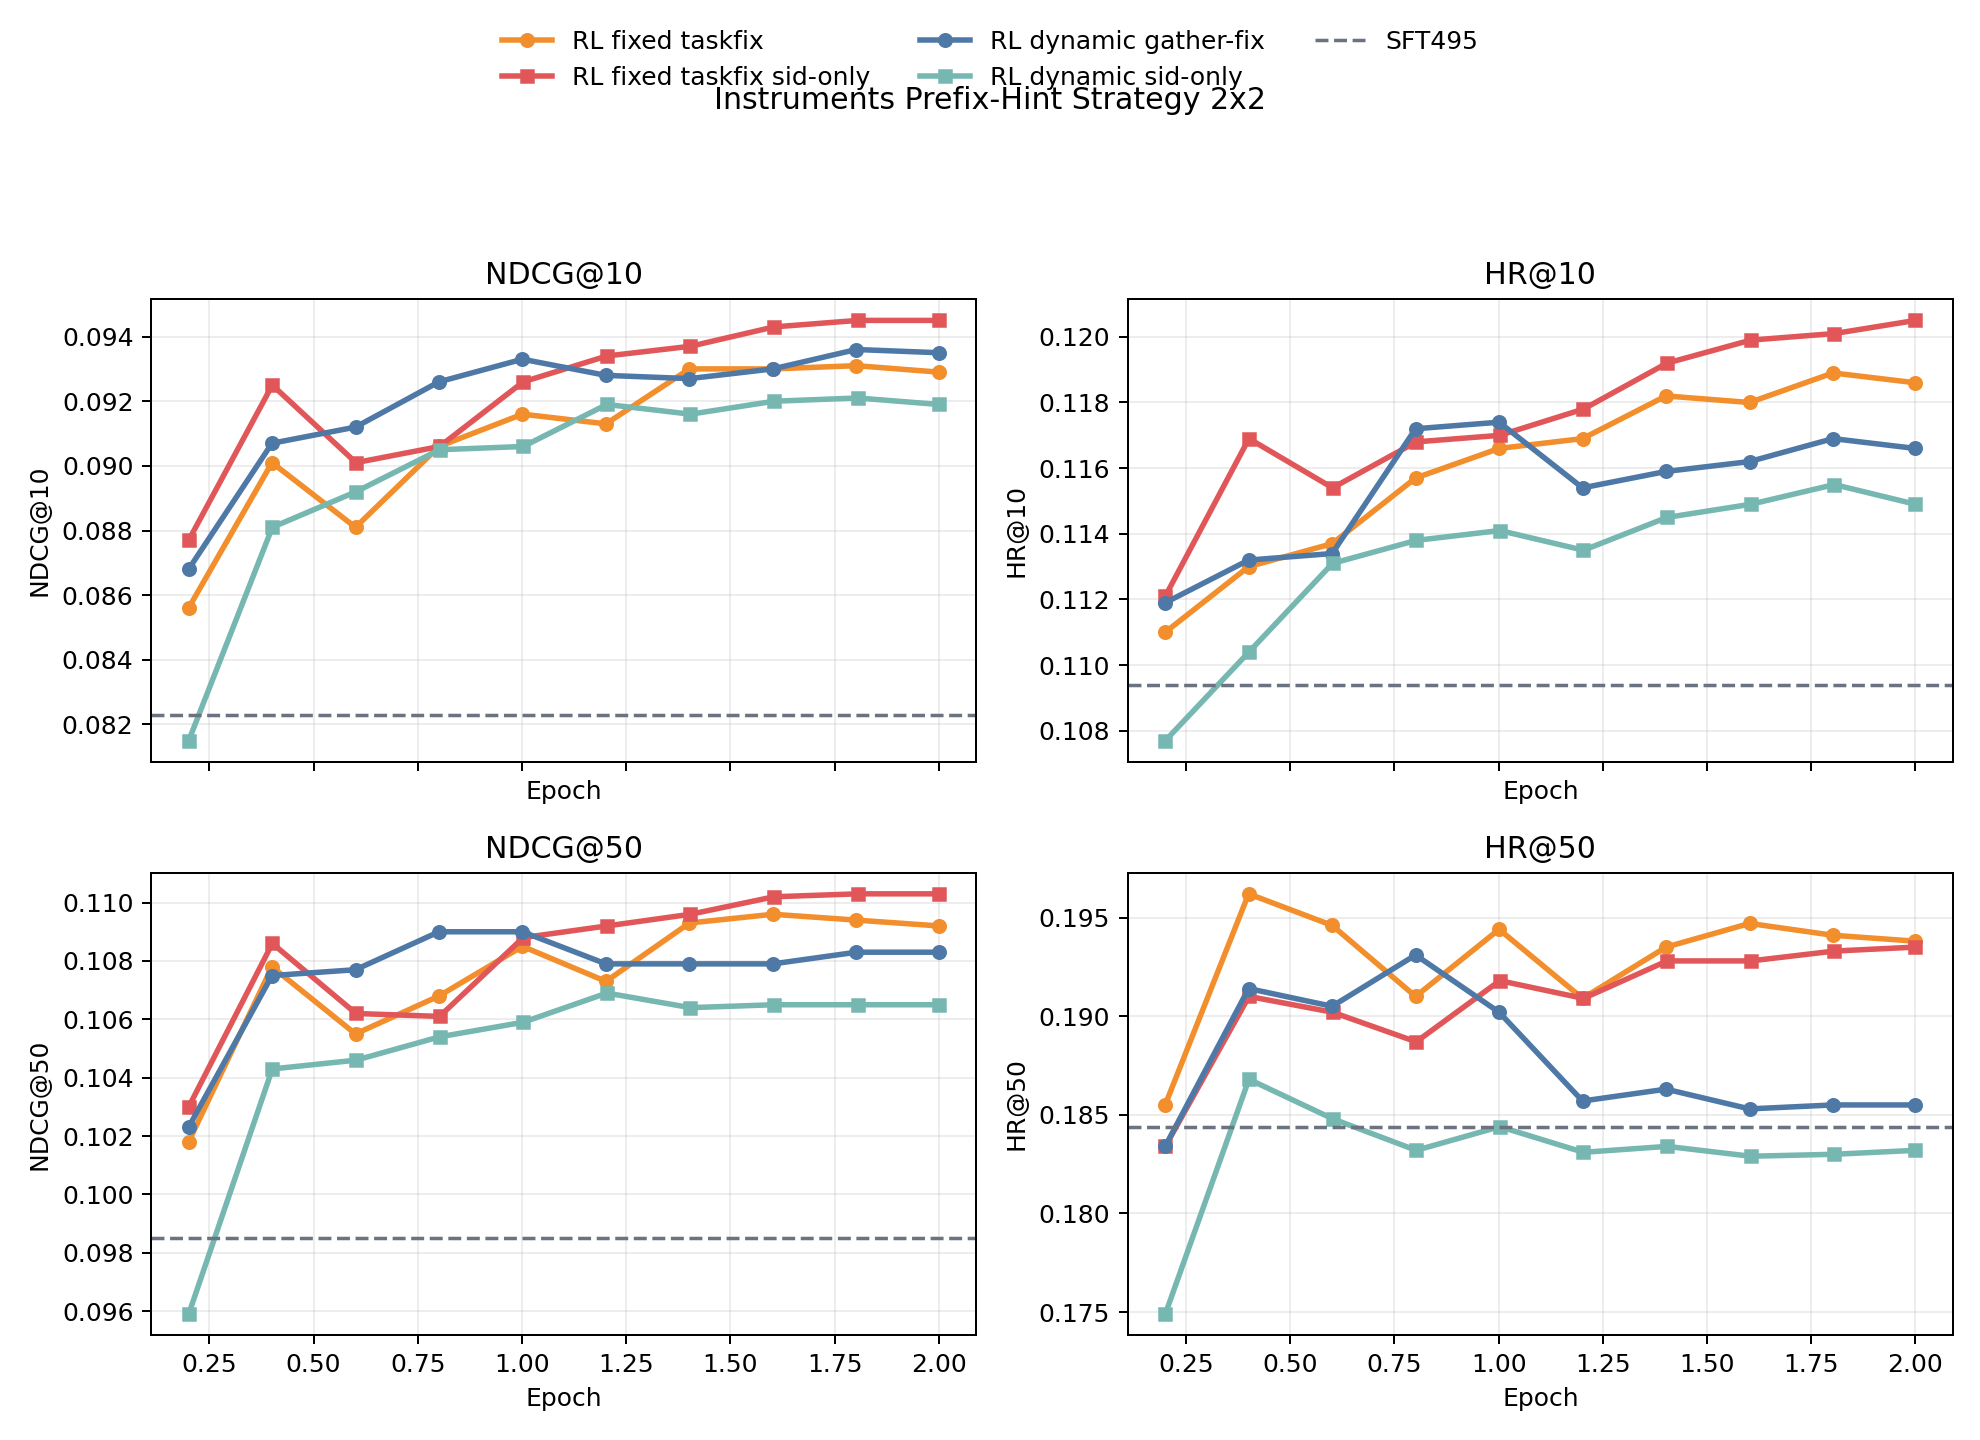
\includegraphics[width=0.96\textwidth]{prefix_hint_strategy_2x2_curves.png}
\caption{prefix-hint 2x2 的完整 epoch 曲线。}
\end{figure}

这组对照可以回答两个更细的问题：

\begin{itemize}
\item 在 adaptive 行里，\texttt{dynamic gather-fix} 四个主指标同时强于 \texttt{dynamic sid-only}，说明 adaptive hinting 本身仍然需要 task-aware prefix，而不是退化成 first-token 就够。
\item 在 fixed 行里，\texttt{fixed taskfix sid-only} 把 \texttt{NDCG@10} 从 \texttt{0.0931} 提到 \texttt{0.0945}，而 \texttt{fixed taskfix} 保住了略高的 \texttt{HR@50}；因此 fixed 侧更像是在 top-10 与 coverage 之间做形状调整，而不是单边支配。
\item 跨行看，当前 best-point 意义下 fixed 侧整体仍强于 adaptive 侧，因此本文后面的 loss/CE 讨论都优先放在 fixed family 上展开。
\end{itemize}

\subsection{RQ2.3 Prefix Budget 敏感性：max1}

如果把 adaptive hint 的在线 budget 从 \texttt{max depth=3} 收紧到 \texttt{1}，可以更直接地回答“hint signal 是否真的来自更深的 prefix”。

\begin{table}[H]
\centering
\small
\setlength{\tabcolsep}{4pt}
\begin{tabular}{p{3.8cm} p{2.4cm} c c c}
\toprule
Variant & Best ckpt & Epoch & NDCG@10 & HR@50 \\
\midrule
rule-only rerun & checkpoint-2997 & 1.802 & 0.0960 & 0.1681 \\
dynamic gather-fix & checkpoint-2997 & 1.802 & 0.0936 & 0.1855 \\
dynamic max1 & checkpoint-1332 & 0.801 & 0.0934 & 0.1905 \\
fixed taskfix sid-only & checkpoint-2652 & 2.000 & 0.0945 & 0.1935 \\
\bottomrule
\end{tabular}
\caption{max1 说明“只给一个 prefix token”依然有信号，但它更像 early-stop candidate。}
\end{table}

\begin{figure}[H]
\centering

\includegraphics[width=0.96\textwidth]{max1-ablation-epoch-curves.png}
\caption{max1 ablation 曲线。}
\end{figure}

\begin{figure}[H]
\centering

\includegraphics[width=0.96\textwidth]{max1-vs-fixed-epoch-curves.png}
\caption{max1 与 dynamic / fixed 参考线的 focused comparison。}
\end{figure}

\begin{itemize}
\item \texttt{max1} 没有退化成 plain \texttt{rule-only}，因为它保住了显著更高的 coverage。
\item 但完整轨迹表明，它的优势主要停在前中段；和 \texttt{dynamic gather-fix} 相比，它更像一个 budget-constrained early-stop 变体，而不是新的 long-run default。
\item 这也反过来说明 RQ2 的主结论不是“任意 prefix 都行”，而是：prefix hint 确实有效，但深度、task awareness 和 fixed/adaptive 交互方式都会改变最终 trade-off 的形状。
\end{itemize}

\section{RQ3: Ablation Study}

\subsection{RQ3.1 训练任务范围消融}

当前可比较的 fixed prefix-hint 训练数据范围可以压成三档：

\begin{itemize}
\item \texttt{ours (3-task)}：\texttt{fixed taskfix}，覆盖 mixed 三任务
\item \texttt{sid-only}：\texttt{fixed taskfix sid-only}
\item \texttt{sid + item-to-index} 两任务近似：当前仓库里已跑出的 \texttt{sid-title-desc} dual-task 线，用来代表缩窄后的 two-task hint scope
\end{itemize}

\begin{table}[H]
\centering
\small
\setlength{\tabcolsep}{4pt}
\begin{tabular}{p{4.1cm} p{2.3cm} c c c}
\toprule
Task scope & Best ckpt & NDCG@10 & HR@10 & HR@50 \\
\midrule
\texttt{3-task} / fixed taskfix & checkpoint-2997 & 0.0931 & 0.1189 & 0.1941 \\
\texttt{sid-only} / fixed sid-only & checkpoint-2652 & 0.0945 & 0.1205 & 0.1935 \\
\texttt{two-task} / fixed dual-task (\texttt{sid-title-desc}) & checkpoint-3012 & 0.0939 & 0.1169 & 0.1905 \\
\bottomrule
\end{tabular}
\caption{训练任务范围消融：当前已完成结果主要来自 fixed prefix-hint family。}
\end{table}

\begin{figure}[H]
\centering
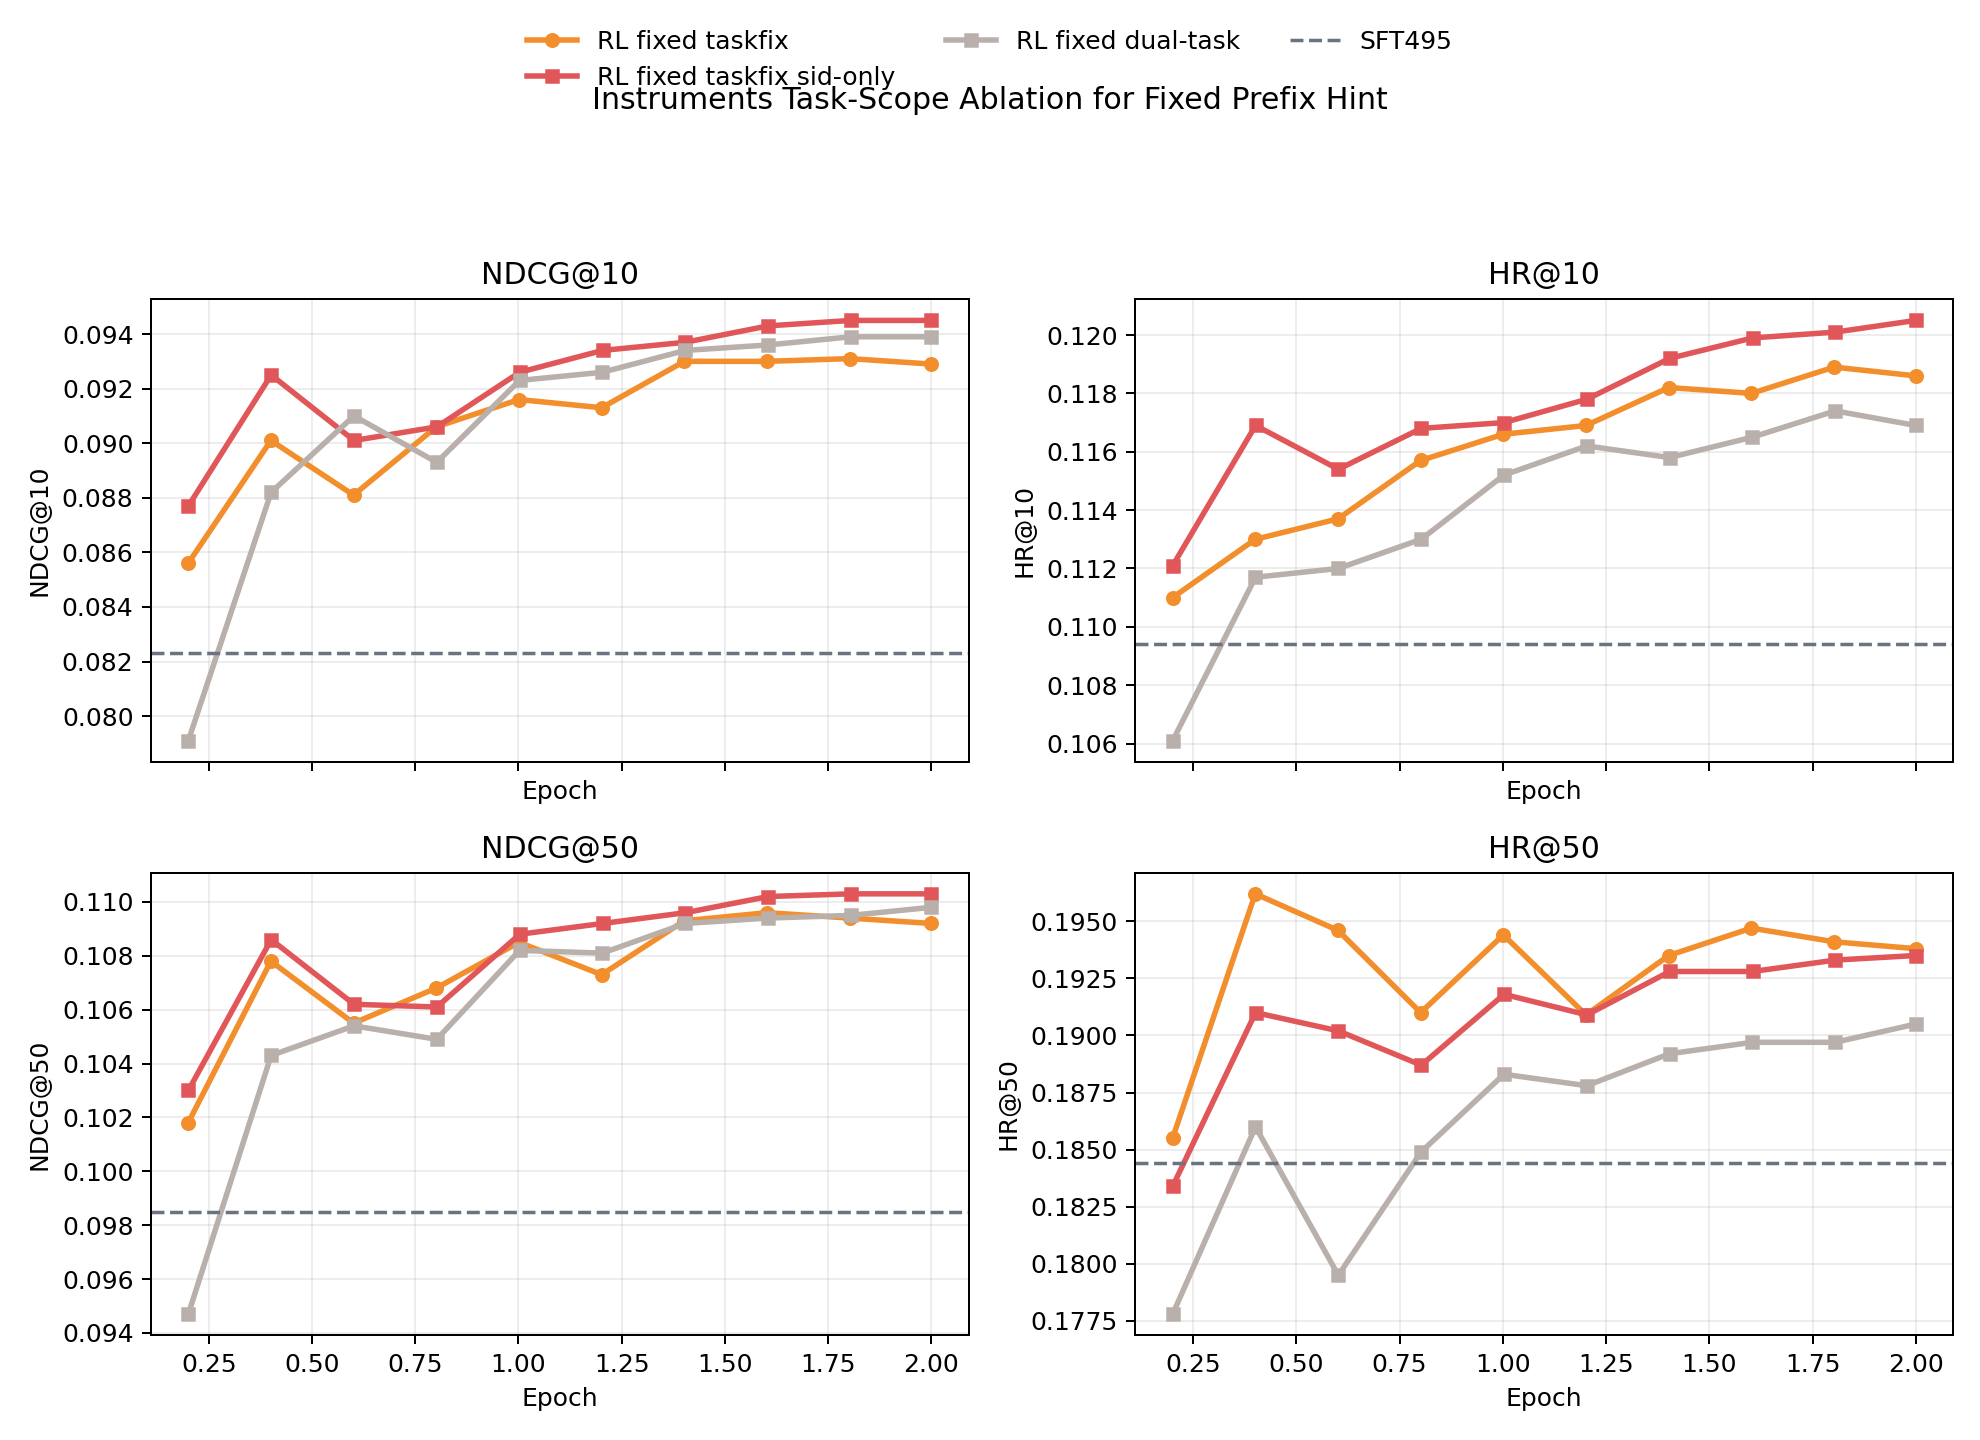
\includegraphics[width=0.96\textwidth]{task_scope_ablation_curves.png}
\caption{3-task / sid-only / two-task 的 fixed prefix-hint task-scope ablation。}
\end{figure}

\begin{itemize}
\item 从 top-10 看，\texttt{sid-only} 当前最强；这说明 first-token setting 在 Instruments 上并不是弱化版。
\item 从 coverage 看，完整 \texttt{3-task} mixed 仍然最稳，\texttt{HR@50=0.1941} 略高于 \texttt{sid-only} 的 \texttt{0.1935}。
\item 当前 two-task 线没有超过前两者，因此现有证据更支持“任务裁剪会改变 trade-off 形状”，而不是“少任务一定更强”。
\end{itemize}

\subsection{RQ3.2 Loss 设计消融}

这一层只看目标函数本身，不再讨论 hint strategy：

\begin{table}[H]
\centering
\footnotesize
\setlength{\tabcolsep}{4pt}
\begin{tabularx}{\textwidth}{p{3.3cm} p{2.1cm} c c Y}
\toprule
Loss design & 代表性 run / 状态 & NDCG@10 & HR@50 & 说明 \\
\midrule
suffix-only GRPO & \texttt{fixed taskfix} & 0.0931 & 0.1941 & 不加 prefix-side SFT / CE，作为 loss baseline \\
prefix SFT + suffix-only GRPO & \texttt{fixed+CE} family & up to 0.0953 & up to 0.1985 & 已完成；其中 \texttt{ce=0.01} 给出更高 top-10，\texttt{ce=0.005} 给出更高 coverage；细节放到 RQ4 展开 \\
full-sequence SFT + GRPO & running & \textemdash & \textemdash & 当前还没有稳定结果可放入主比较表 \\
\bottomrule
\end{tabularx}
\caption{loss 层面当前可比较的三种设定。}
\end{table}

当前 running 的 full-sequence 线对应 launcher：\path{hope/Instruments-genrec/rl_fixed_full_sequence_sft.sh}。

这张表对应的结论目前也比较明确：

\begin{itemize}
\item 一旦在 suffix-only GRPO 旁边加入 prefix-side SFT/CE，frontier 就已经发生了可观测变化，否则不会同时看到 \texttt{0.0953} 级别的 top-10 和 \texttt{0.1985} 级别的 coverage 峰值。
\item 但“fixed + CE”现在还不是单一点，而是一条 coefficient family；因此它在 RQ3 里只能先回答“这个 loss 方向是否有用”，更细的最优系数判断交给 RQ4。
\item full-sequence SFT + GRPO 目前还处在 running 状态，所以这轮重构只把它明确标进问题定义，不提前写结论。
\end{itemize}

\section{RQ4: 分析后训练中 CE Loss 的影响}

\subsection{RQ4 的比较对象}

这一节只讨论 fixed prefix-hint family 里的后训练 CE 系数，不把 dynamic CE trajectory 混进主表。对两个数据集，统一比较四条线：

\begin{itemize}
\item non-CE baseline：plain \texttt{fixed taskfix}
\item \texttt{CE=0.001}
\item \texttt{CE=0.005}
\item \texttt{CE=0.01}
\end{itemize}

因此 RQ4 回答的不是“加不加 CE”，而是“加了 CE 之后，系数怎么改变 top-10 / coverage 的形状，而且这种变化在 Instruments 与 Arts 上是否一致”。

\subsection{Instruments：0.005 提升 coverage，0.01 提升 long-run top-10}

\begin{table}[H]
\centering
\small
\setlength{\tabcolsep}{4pt}
\begin{tabular}{p{3.6cm} p{2.2cm} c c c c}
\toprule
Variant & Best ckpt & NDCG@10 & HR@10 & NDCG@50 & HR@50 \\
\midrule
fixed taskfix (no CE) & checkpoint-2997 & 0.0931 & 0.1189 & 0.1094 & 0.1941 \\
\texttt{CE=0.001} & checkpoint-2664 & 0.0931 & 0.1168 & 0.1102 & 0.1951 \\
\texttt{CE=0.005} & checkpoint-1665 & 0.0945 & 0.1180 & 0.1118 & 0.1985 \\
\texttt{CE=0.01} & checkpoint-2997 & 0.0953 & 0.1204 & 0.1113 & 0.1943 \\
\bottomrule
\end{tabular}
\caption{Instruments 上的 fixed CE coefficient sweep。}
\end{table}

\begin{figure}[H]
\centering
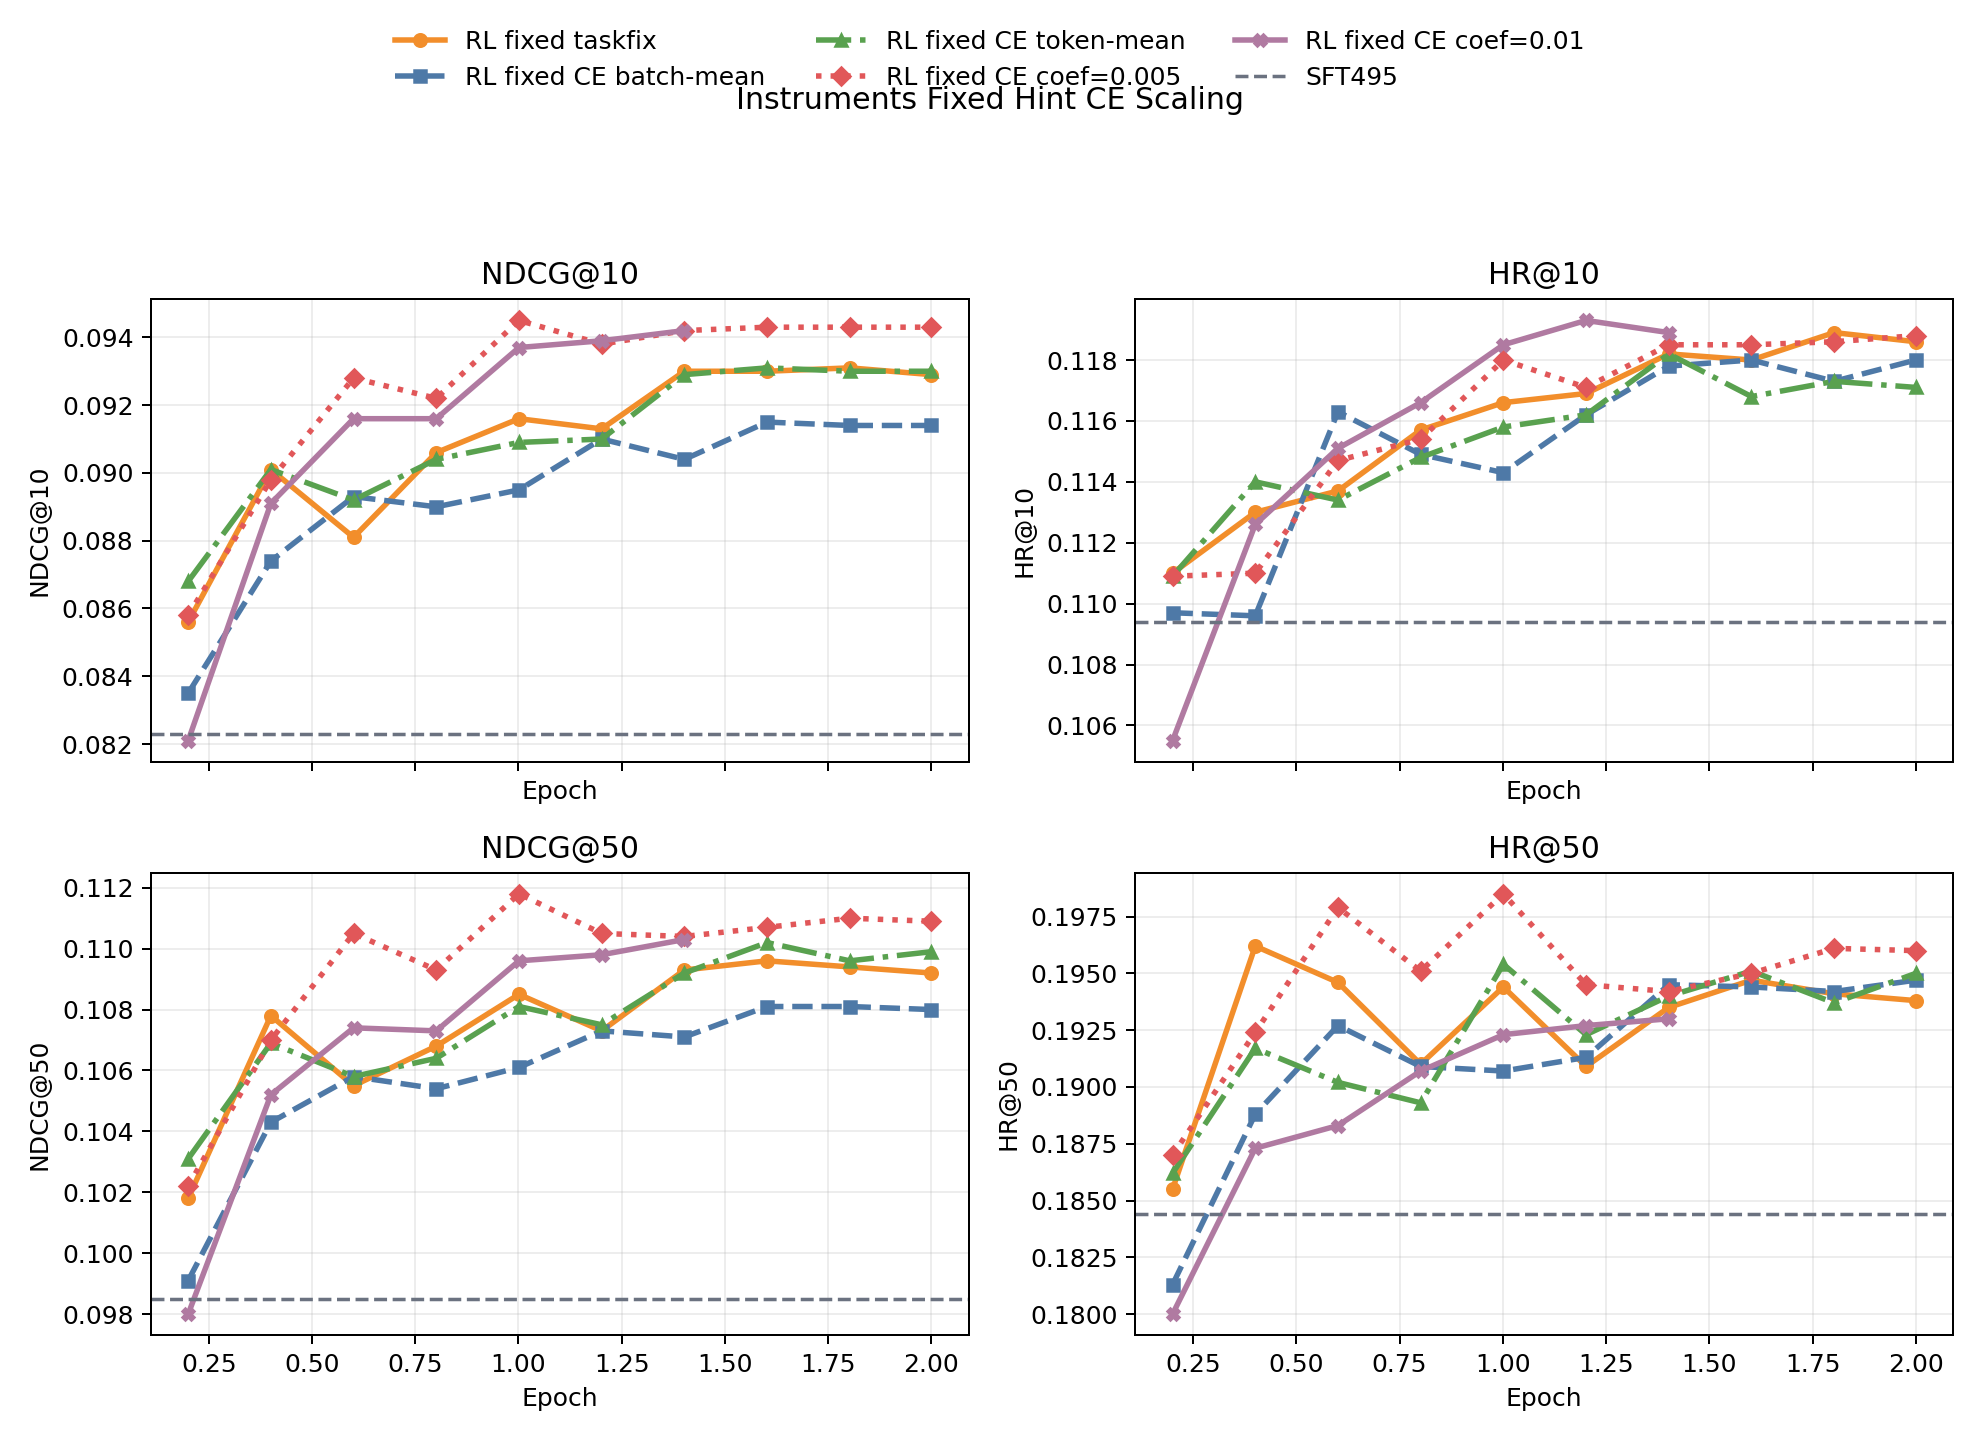
\includegraphics[width=0.96\textwidth]{ce_scaling_three_variants_curves.png}
\caption{Instruments 上 fixed CE coefficient 的完整曲线。}
\end{figure}

\begin{itemize}
\item \texttt{CE=0.001} 更像一个温和正则：\texttt{NDCG@10} 基本不变，但 \texttt{HR@50} 从 \texttt{0.1941} 提到 \texttt{0.1951}。
\item \texttt{CE=0.005} 是当前 coverage 最强点，\texttt{HR@50} 来到 \texttt{0.1985}，同时 \texttt{NDCG@10} 也升到 \texttt{0.0945}。
\item \texttt{CE=0.01} 则把 best \texttt{NDCG@10} 继续抬到 \texttt{0.0953}，而且 best 点回到更晚的 \texttt{checkpoint-2997}；它更像“long-run top-10 强化”，而不是 coverage 最优。
\end{itemize}

\subsection{Arts：0.001 的 coverage 最强，但 0.005 更稳地保住 headline}

\begin{table}[H]
\centering
\small
\setlength{\tabcolsep}{4pt}
\begin{tabular}{p{3.6cm} p{2.2cm} c c c c}
\toprule
Variant & Best ckpt & NDCG@10 & HR@10 & NDCG@50 & HR@50 \\
\midrule
fixed taskfix (no CE) & checkpoint-3368 & 0.0956 & 0.1248 & 0.1120 & 0.2007 \\
\texttt{CE=0.001} & checkpoint-2105 & 0.0943 & 0.1244 & 0.1114 & 0.2029 \\
\texttt{CE=0.005} & checkpoint-2105 & 0.0956 & 0.1257 & 0.1118 & 0.2006 \\
\texttt{CE=0.01} & checkpoint-2105 & 0.0941 & 0.1228 & 0.1106 & 0.1990 \\
\bottomrule
\end{tabular}
\caption{Arts 上的 fixed CE coefficient sweep。}
\end{table}

\begin{figure}[H]
\centering
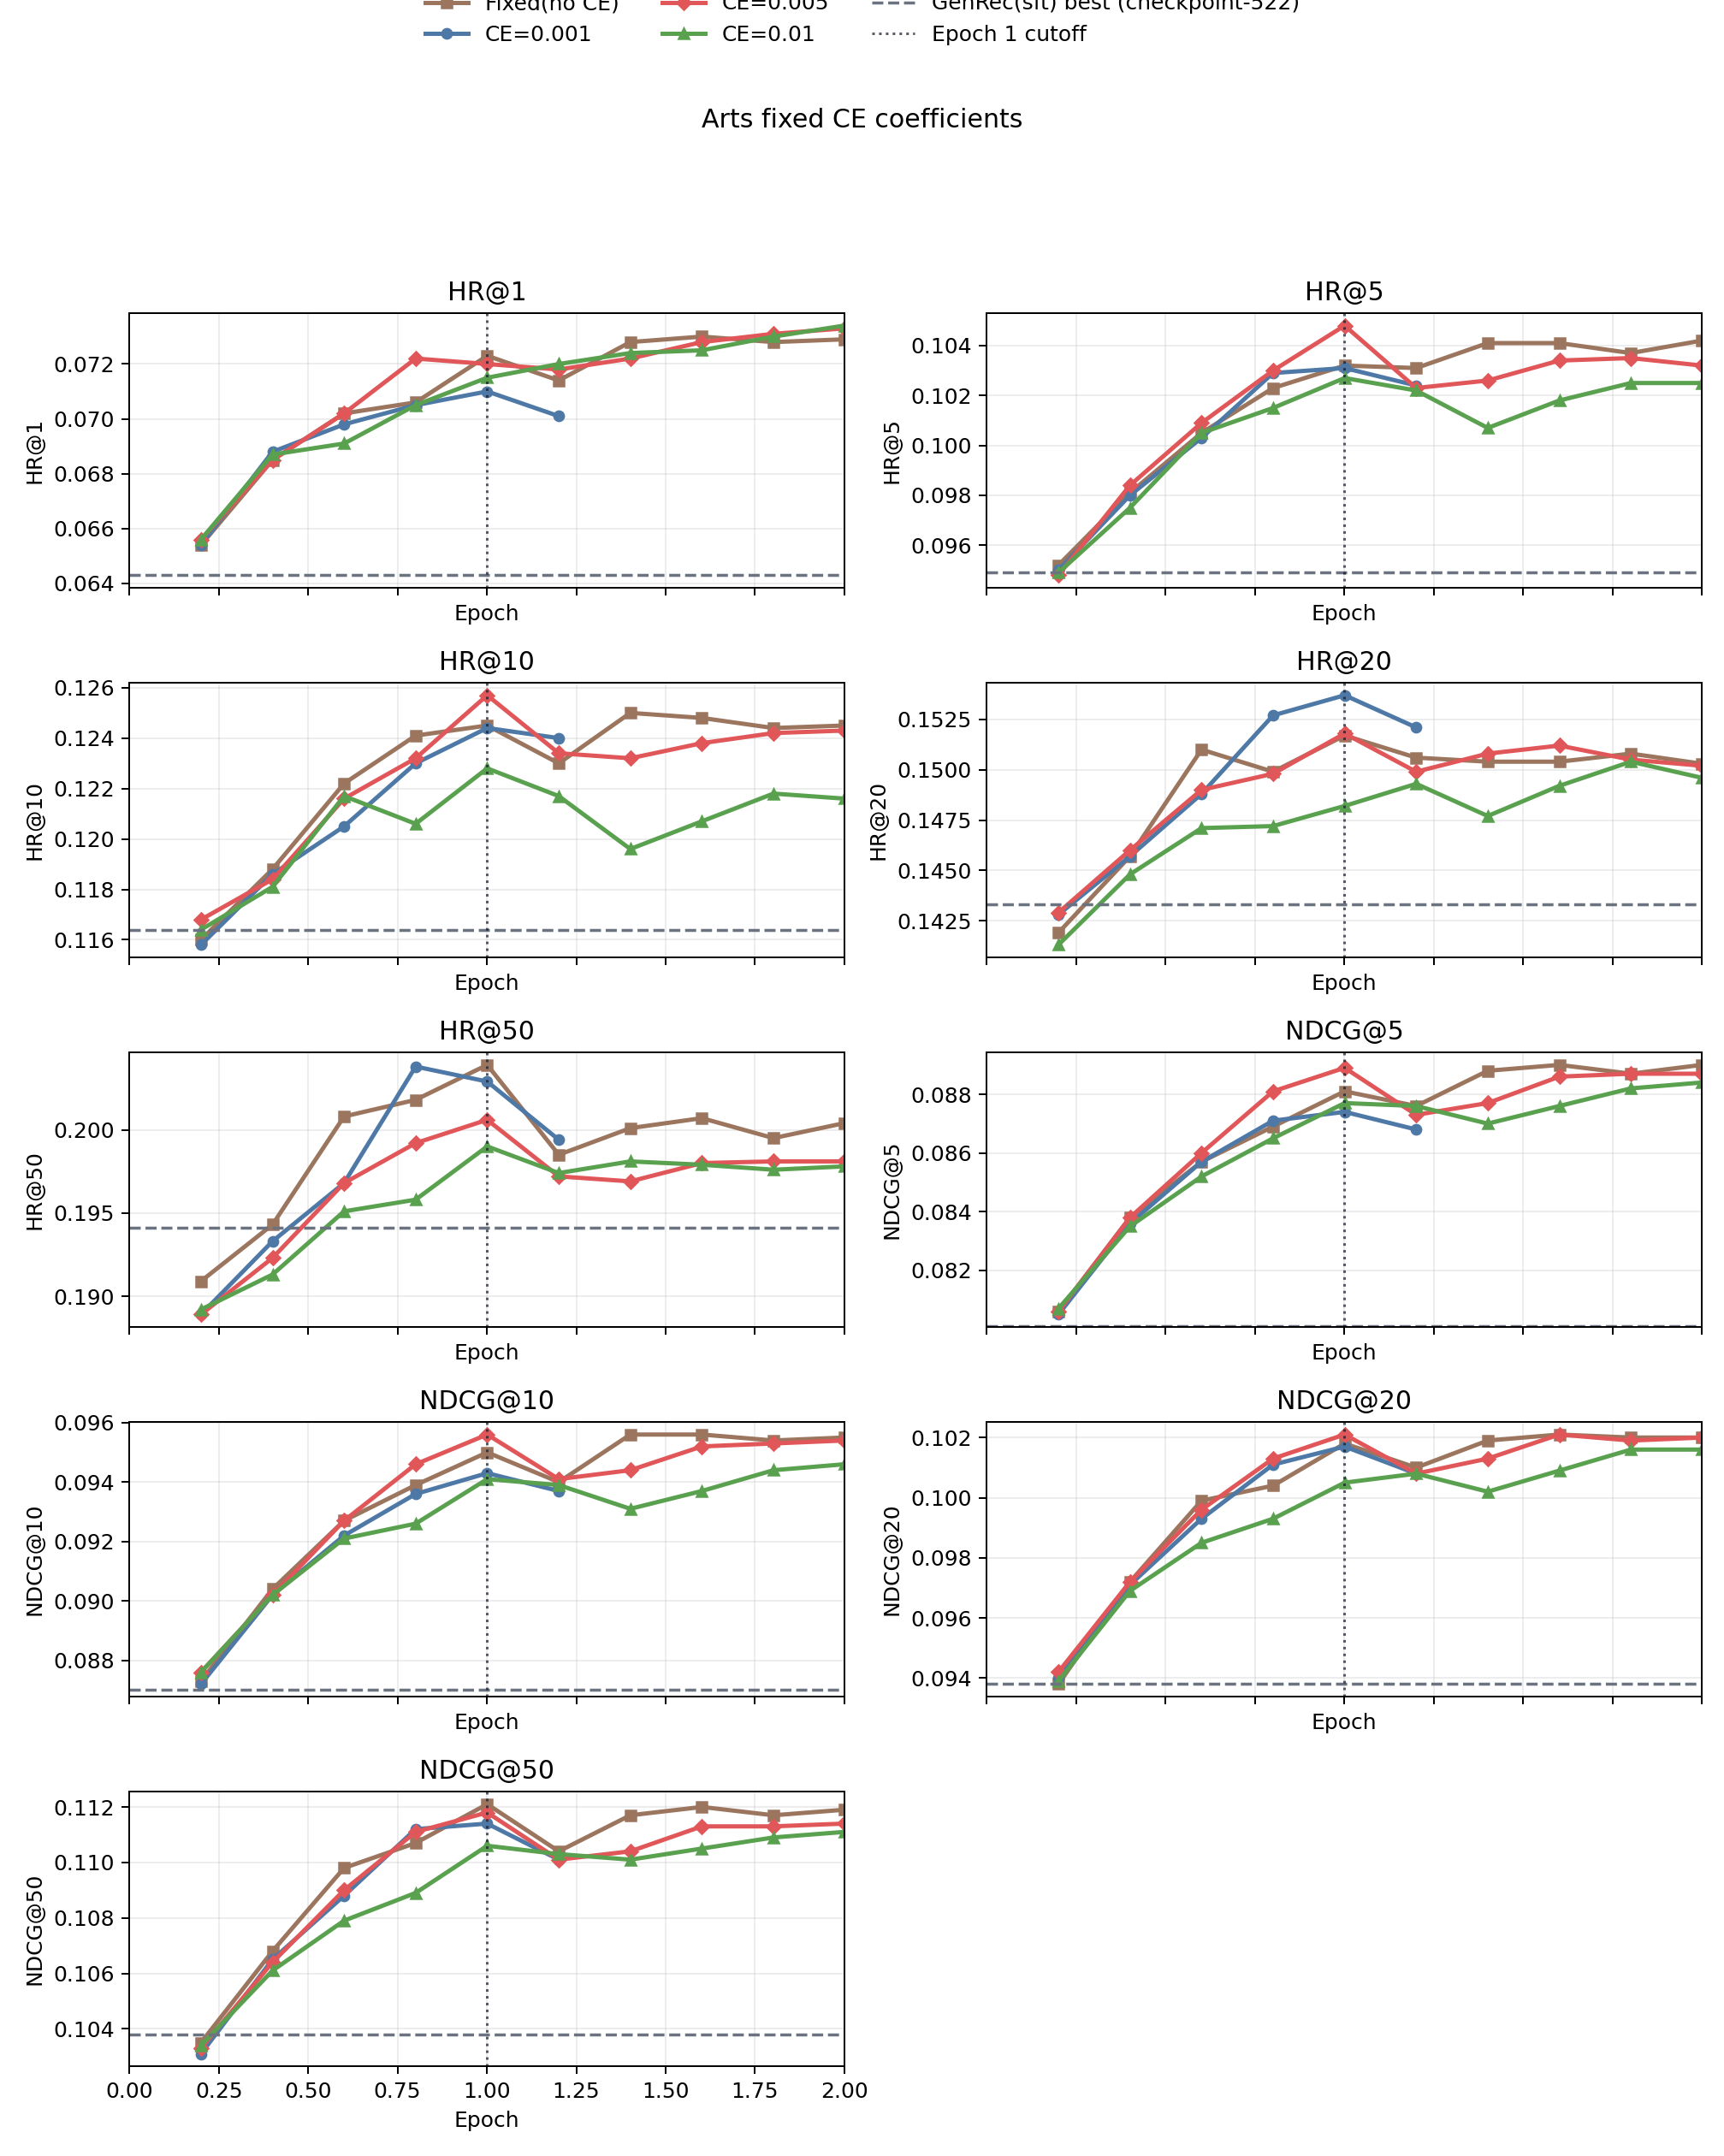
\includegraphics[width=0.96\textwidth]{genrec-only-arts-fixed-ce-coefficients-curves.png}
\caption{Arts 上 fixed CE coefficient 的完整曲线。}
\end{figure}

\begin{itemize}
\item Arts 上最明显的 coverage 增益来自 \texttt{CE=0.001}：\texttt{HR@50} 从 \texttt{0.2007} 提到 \texttt{0.2029}，但 top-10 略有回落。
\item \texttt{CE=0.005} 则保住了和 non-CE baseline 持平的 \texttt{NDCG@10=0.0956}，同时把 \texttt{HR@10} 拉到四条线里最高的 \texttt{0.1257}。
\item \texttt{CE=0.01} 在 Arts 上反而没有复制 Instruments 的 long-run top-10 优势，因此它更像一个数据集敏感的高倍率设定。
\end{itemize}

\subsection{跨数据集读法}

\begin{table}[H]
\centering
\small
\begin{tabular}{p{2.2cm} p{3.0cm} p{3.0cm} p{5.0cm}}
\toprule
Dataset & best top-10 coefficient & best coverage coefficient & 读法 \\
\midrule
Instruments & \texttt{CE=0.01} & \texttt{CE=0.005} & 更高倍率会把 top-10 往长跑尾段抬，但 coverage 峰值仍出现在中等系数 \\
Arts & \texttt{CE=0.005} 与 no-CE 并列 & \texttt{CE=0.001} & 较小系数更像 coverage regularizer；过大的 \texttt{0.01} 会同时伤到 top-10 和 coverage \\
\bottomrule
\end{tabular}
\caption{CE 系数的跨数据集 summary。}
\end{table}

因此，RQ4 的主结论不是“存在一个在所有数据集都最优的 CE 系数”，而是：

\begin{itemize}
\item CE 确实会系统性改变 fixed prefix-hint family 的后训练轨迹；
\item 但它改变的是 top-10 与 coverage 的形状，而不是单调地“系数越大越好”；
\item 当前最稳妥的说法是：\texttt{0.005} 更像跨数据集都还站得住的中间档，\texttt{0.01} 更像 Instruments 特有的 top-10 aggressive setting，\texttt{0.001} 则更像 Arts 上的 mild coverage regularizer。
\end{itemize}


\section{结论与下一步}

\subsection{按 RQ 压缩后的主结论}

\begin{enumerate}
\item RQ1：\texttt{rule-only} 仍然定义了当前无 hint top-10 baseline，但真正的 performance frontier 已经转移到 hint-enabled family，尤其是 clean fixed family 与后续 CE variants。
\item RQ2：prefix hint 的训练信号是有效的；在 adaptive 行里，task-aware prefix 明显优于 first-token prefix；在 fixed 行里，task-aware 与 first-token 更像是在交换 top-10 和 coverage，而不是简单单边支配；\texttt{max1} 则说明单 token hint 仍有信号，但更像 early-stop candidate。
\item RQ3：训练任务范围会显著改变 fixed family 的形状，当前最强 top-10 来自 \texttt{sid-only}，最稳 coverage 仍在完整 \texttt{3-task}；loss 侧加入 prefix SFT/CE 已经明确改变 frontier，但 full-sequence SFT + GRPO 还需要等待真实结果。
\item RQ4：CE 系数不会单调地产生收益。当前 \texttt{0.005} 是更稳的中间档，\texttt{0.01} 更像 Instruments 上的 aggressive top-10 设定，而 Arts 对大系数更敏感。
\end{enumerate}

\subsection{下一步最值得补的证据}

\begin{itemize}
\item 等 \path{hope/Instruments-genrec/rl_fixed_full_sequence_sft.sh} 跑完，把 RQ3 的 loss comparison 从“问题定义 + 当前 readout”升级成真正的三线定量比较。
\item 如果后面要选一个固定主配置继续扩数据集，当前最值得优先验证的是 \texttt{fixed taskfix sid-only}、\texttt{hintce-3} 和 \texttt{hintce-4} 的跨数据集稳定性。
\item 对 RQ2，如果后面还要继续讲 prefix hint 机制，优先补的是 task-level readout，而不是再堆更多 headline checkpoint。
\end{itemize}

\clearpage
\appendix

\section{错版 Fixed vs Corrected Fixed}

\subsection{Bug 图}

\begin{figure}[H]
\centering

\includegraphics[width=0.92\textwidth]{fixed-hint-bug-task-depth-distribution.png}
\caption{old fixed 的 bug 会把不同任务的 hint depth 分布系统性压歪。}
\end{figure}

\subsection{任务级摘要}

\begin{table}[H]
\centering
\small
\setlength{\tabcolsep}{4pt}
\begin{tabular}{p{3.2cm} c c c p{4.1cm}}
\toprule
Task & Changed rate & Avg depth correct & Avg depth buggy & 主效应 \\
\midrule
\texttt{task1\_sid\_sft} & 7.64\% & 1.048 & 0.938 & 只被轻微压浅 \\
\texttt{task4\_hisTitle2sid} & 82.35\% & 1.533 & 0.188 & hardest task 几乎被压成 depth-0 \\
\texttt{task5\_title\_desc2sid} & 19.41\% & 0.519 & 0.245 & 一部分 depth-2 被压回 0/1 \\
\bottomrule
\end{tabular}
\caption{old fixed 的 bug 不是“hint 更准”，而是把任务分布系统性压浅。}
\end{table}

\subsection{结论}

\begin{itemize}
\item old fixed 的表面优势，不是来自更正确的 hint map，而是因为 hardest task 被系统性少给 hint。
\item 因此它更像一个带偏置的历史现象学上界，而不是应该继续复用的方法定义。
\item 这也是为什么本文后文在需要 fixed reference 时，默认优先引用 corrected \texttt{fixed taskfix sid-only}。
\end{itemize}

\section{Single-Hint Mixed 消融}

\subsection{实验定义}

这条线现在已经有 fixed / dynamic 两个版本，它们的共同点都不是“只训练 \texttt{task1}”，而是 mixed 三任务仍然一起训练，只把 hint 限制到 \texttt{task1\_sid\_sft}：

\begin{itemize}
\item fixed single-hint mixed：只对 \texttt{task1\_sid\_sft} 注入 fixed hint，其余任务继续按 zero-hint 路径走。
\item dynamic single-hint mixed：只对 \texttt{task1\_sid\_sft} 开 dynamic cascade，其余任务被强制停在 stage-0 / no-hint 路径。
\end{itemize}

\subsection{对应脚本}

{\footnotesize
\begin{itemize}
\item 画图脚本：\path{docs/research/scripts/build_instruments_report_figures.py}
\item 脚本目录：\path{hope/Qwen2_5-3B-Isntruct-qwen4B-4-256-MIMIGenRec-grec/}
\item fixed launcher：\path{Qwen2_5-3B-Isntruct-qwen4B-4-256-MIMIGenRec-grec-rl-rule-only-fixed-hint-sid-hint-only-mixed.sh}
\item dynamic launcher：\path{Qwen2_5-3B-Isntruct-qwen4B-4-256-MIMIGenRec-grec-rl-rule-only-dynamic-hint-sid-hint-only-mixed.sh}
\end{itemize}
}

\subsection{关键指标}

\begin{table}[H]
\centering
\small
\setlength{\tabcolsep}{4pt}
\begin{tabular}{p{3.8cm} p{2.2cm} c c c p{2.4cm}}
\toprule
Variant & Best ckpt & Epoch & NDCG@10 & HR@50 & 备注 \\
\midrule
fixed taskfix & checkpoint-2997 & 1.802 & 0.0931 & 0.1941 & clean fixed 参考 \\
fixed taskfix sid-only & checkpoint-2652 & 2.000 & 0.0945 & 0.1935 & clean sid-only 上界 \\
old fixed mixed-single & checkpoint-3326 & 2.000 & 0.0953 & 0.1938 & 带 bug caveat 的历史上界 \\
fixed single-hint mixed & checkpoint-2664 & 1.602 & 0.0948 & 0.1958 & 当前最强 partial-hint 候选 \\
dynamic dual-task & checkpoint-1510 & 1.003 & 0.0930 & 0.1885 & 当前 task-filtered dynamic 参考 \\
dynamic single-hint mixed & checkpoint-2331 & 1.402 & 0.0911 & 0.1823 & 当前已同步到 checkpoint-2997，但仍弱于 dynamic baseline \\
\bottomrule
\end{tabular}
\caption{single-hint mixed 现在已经从 fixed-only 读法扩展到 fixed / dynamic 两个版本。}
\end{table}

\subsection{图表}

\begin{figure}[H]
\centering

\includegraphics[width=0.96\textwidth]{single_hint_vs_fixed_family_epoch_curves.png}
\caption{single-hint mixed vs fixed family。}
\end{figure}

\begin{figure}[H]
\centering
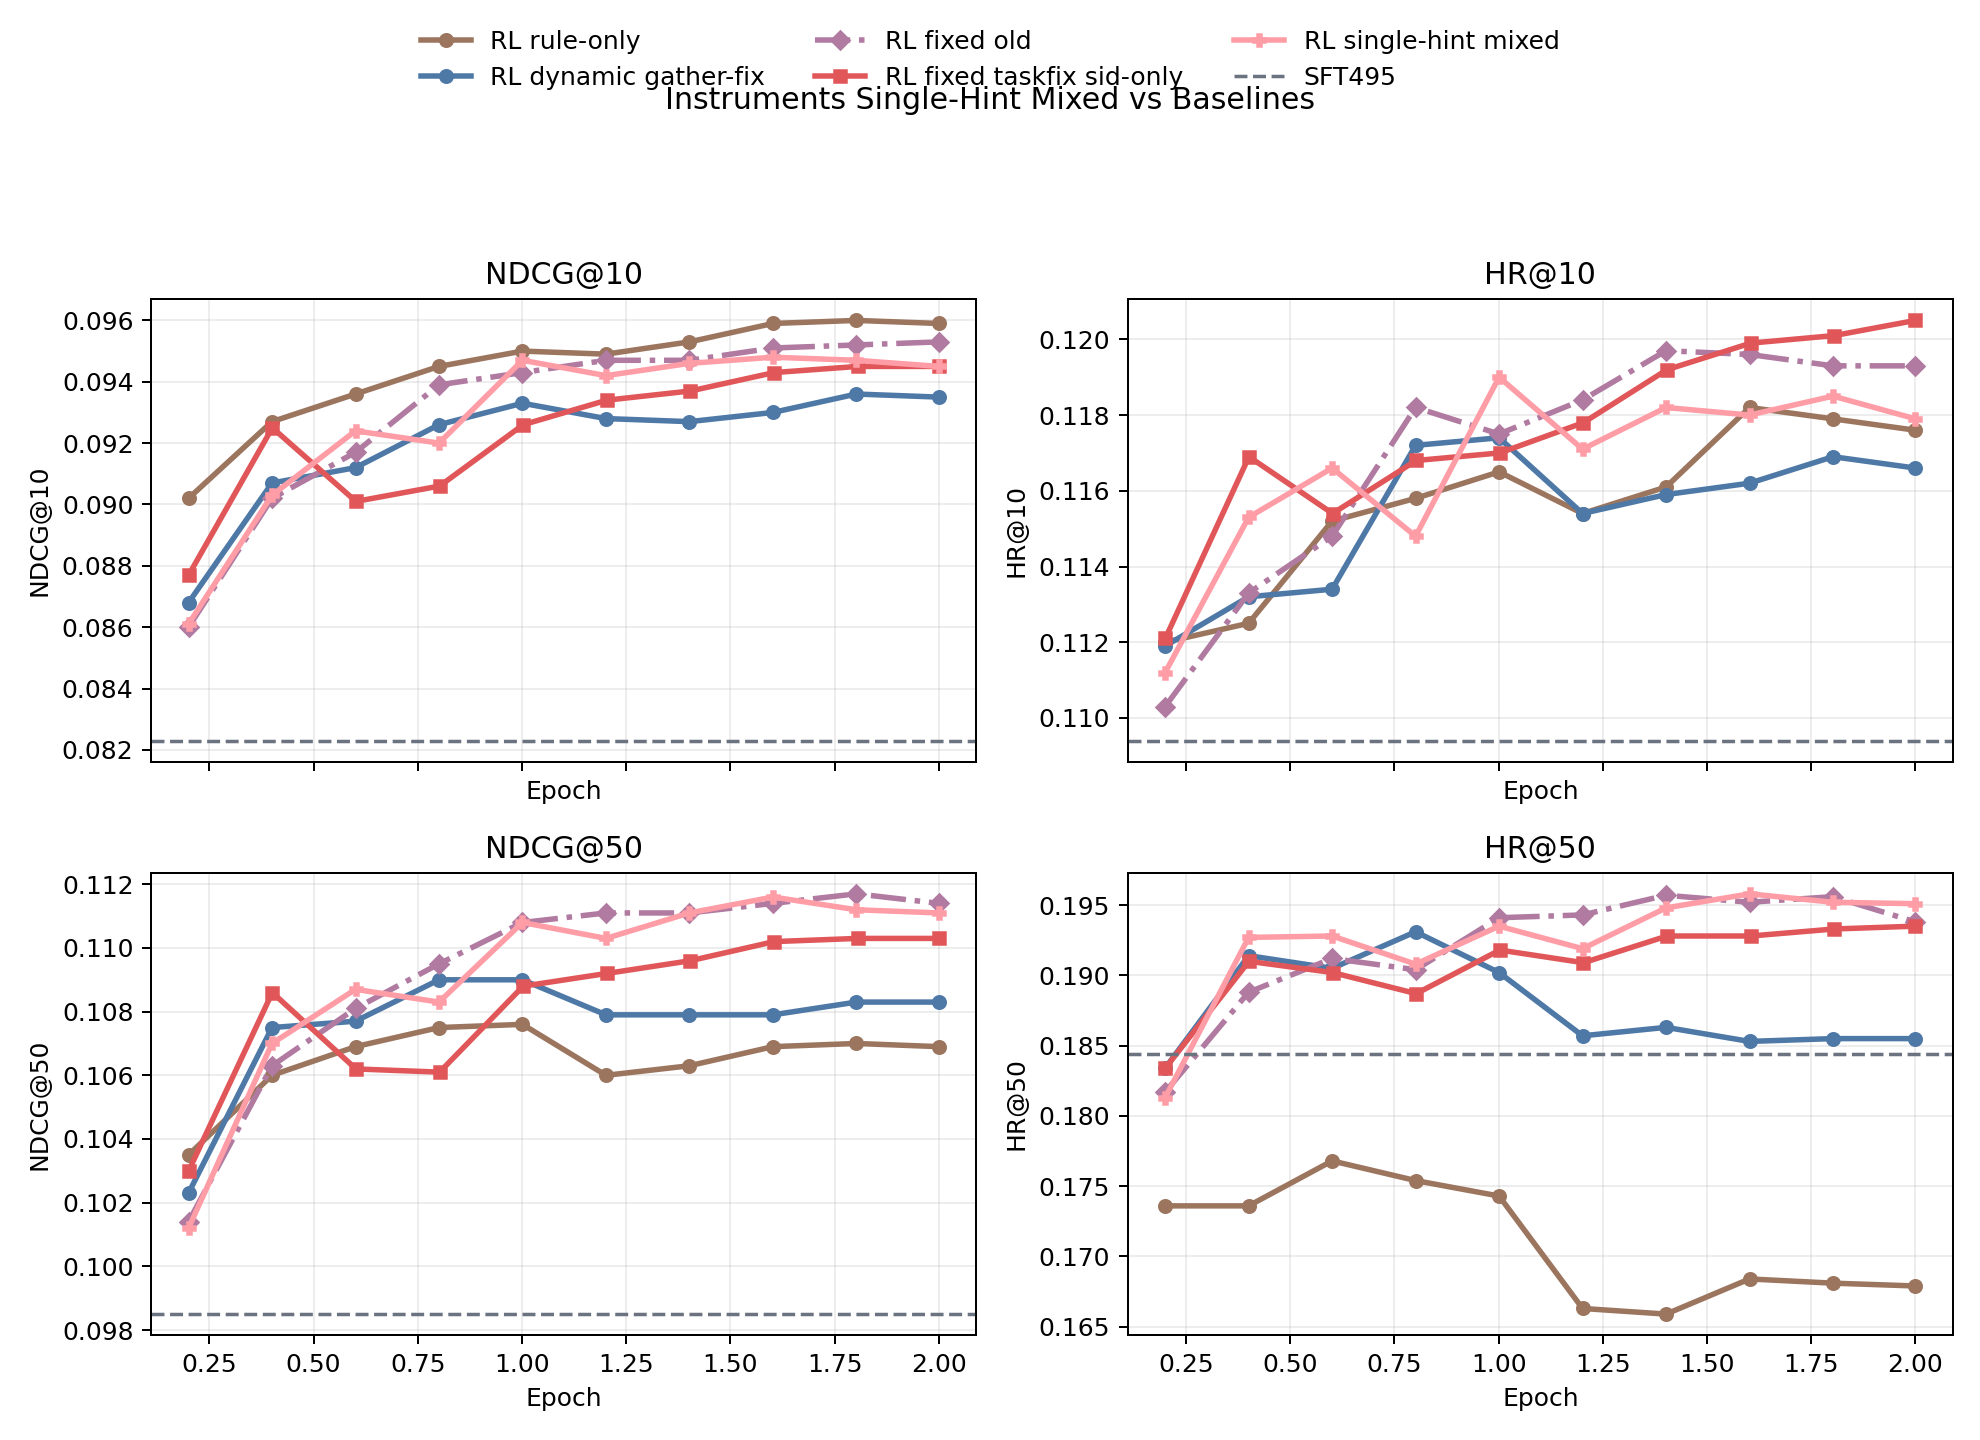
\includegraphics[width=0.96\textwidth]{single_hint_mixed_vs_baselines_compact_curves.png}
\caption{single-hint mixed vs dynamic family；当前 compact 图里直接放入新的 dynamic single-hint mixed。}
\end{figure}

\subsection{结论}

\begin{itemize}
\item 这条线不再只是 fixed-only 实验；现在已经能把 fixed / dynamic 两个“只对 \texttt{task1} 给 hint”的版本放到同一节里读。
\item fixed single-hint mixed 仍然是当前更强、更完整的 partial-hint 候选：它的 best 点已经同时超过 corrected \texttt{fixed taskfix sid-only} 的 \texttt{NDCG@10} 和 \texttt{HR@50}。
\item dynamic single-hint mixed 现在已经补到 \texttt{checkpoint-2997}。它的 best \texttt{NDCG@10} 点在 \texttt{checkpoint-2331 / 0.0911}，对应 \texttt{HR@50=0.1823}；peak \texttt{HR@50} 则出现在 \texttt{checkpoint-1665 / 0.1874}，而尾点回落到 `0.0905 / 0.1802`。
\item 这意味着之前在 \texttt{checkpoint-666} 看起来还算有希望的 early-window readout，并没有沿着长跑继续长成一个真正的 dynamic 候选。按当前完整得多的轨迹看，它既没有接近 fixed \texttt{single-hint mixed}，也没有超过 canonical \texttt{dynamic gather-fix} 或 \texttt{dynamic dual-task}。
\item 因而这条线现在更像“帮助理解 partial-hint 机制边界”的对照项，而不是需要优先追加资源的新主候选。真正仍值得继续解释的 partial-hint 故事，仍然主要发生在 fixed \texttt{single-hint mixed} 上。
\end{itemize}

\section{Single-Hint Mixed + CE(0.005) 完整轨迹}

\subsection{实验定义}

这条新线把前一节的 fixed \texttt{single-hint mixed} 和 CE scaling 里的
\texttt{hintce-3} 直接拼到一起：

\begin{itemize}
\item 训练任务仍然保持 mixed 三任务。
\item hint 仍然只对 \texttt{task1\_sid\_sft} 打开，也就是沿用 \texttt{single-hint mixed} 的 partial-hint 设定。
\item 同时在这个设定上再加 fixed-side prompt CE，倍率沿用 \texttt{0.005}，也就是和 \texttt{hintce-3} 相同的 CE 系数。
\end{itemize}

因此这里最自然的比较对象不是整个 fixed family，而是它的两个“父实验”：
\texttt{single-hint mixed} 和 fixed CE coef=\texttt{0.005}（\texttt{hintce-3}）。

\subsection{对应脚本}

{\footnotesize
\begin{itemize}
\item 画图脚本：\path{docs/research/scripts/build_instruments_report_figures.py}
\item 脚本目录：\path{hope/Qwen2_5-3B-Isntruct-qwen4B-4-256-MIMIGenRec-grec/}
\item plain single-hint mixed launcher：\path{Qwen2_5-3B-Isntruct-qwen4B-4-256-MIMIGenRec-grec-rl-rule-only-fixed-hint-sid-hint-only-mixed.sh}
\item single-hint mixed + CE(0.005) launcher：\path{Qwen2_5-3B-Isntruct-qwen4B-4-256-MIMIGenRec-grec-rl-rule-only-fixed-hint-sid-hint-only-mixed-hint-ce.sh}
\item fixed CE coef=\texttt{0.005} parent launcher：\path{Qwen2_5-3B-Isntruct-qwen4B-4-256-MIMIGenRec-grec-rl-rule-only-fixed-hint-ce.sh}
\end{itemize}
}

\subsection{关键指标}

\begin{table}[H]
\centering
\small
\setlength{\tabcolsep}{4pt}
\begin{tabular}{p{4.2cm} p{2.2cm} c c c p{2.3cm}}
\toprule
Variant & Best ckpt & Epoch & NDCG@10 & HR@50 & 备注 \\
\midrule
fixed single-hint mixed & checkpoint-2664 & 1.602 & 0.0948 & 0.1958 & plain partial-hint baseline \\
fixed CE coef=0.005 (\texttt{hintce-3}) & checkpoint-1665 & 1.001 & 0.0945 & 0.1985 & plain CE parent line \\
single-hint mixed + CE(0.005) & checkpoint-2664 & 1.602 & 0.0943 & 0.1919 & 当前已同步到 checkpoint-3326 \\
\bottomrule
\end{tabular}
\caption{single-hint mixed + CE(0.005) 与两个 parent line 的完整轨迹对照。}
\end{table}

\subsection{图表}

\begin{figure}[H]
\centering
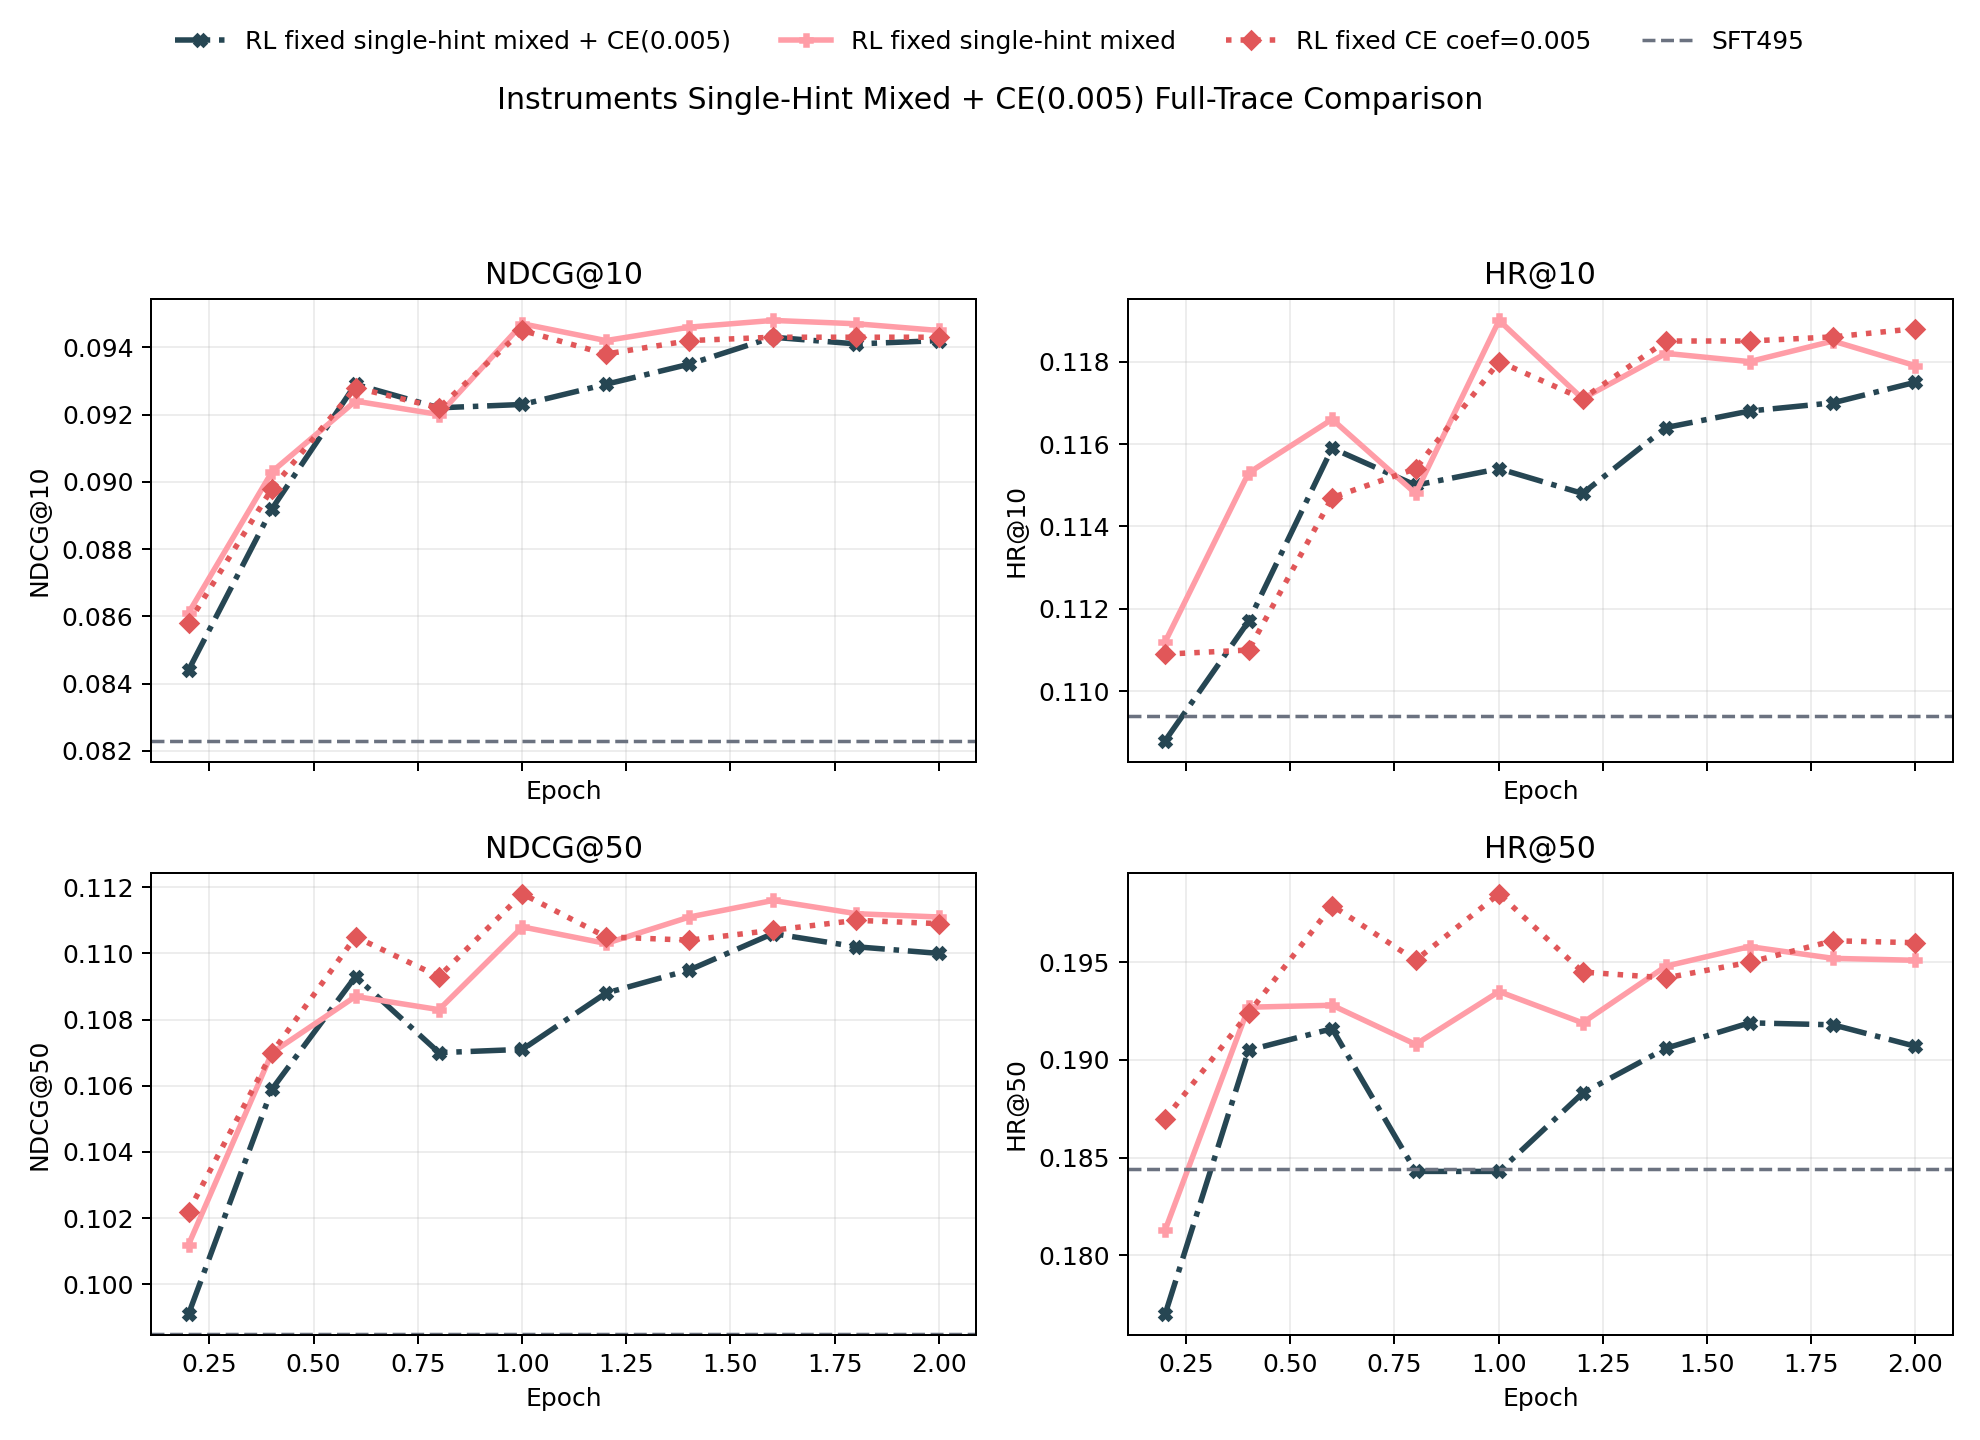
\includegraphics[width=0.96\textwidth]{single_hint_mixed_ce005_vs_parents_curves.png}
\caption{single-hint mixed + CE(0.005) vs plain single-hint mixed vs fixed CE coef=\texttt{0.005}。}
\end{figure}

\subsection{结论}

\begin{itemize}
\item 这条线现在虽然已经补齐到完整 \texttt{checkpoint-3326}，但按代码实现看，它并不是一个“把 \texttt{single-hint mixed} 和 \texttt{hintce-3} 直接做加法”的 clean additive ablation。
\item 关键原因在于 task scope 被改了两次：这两个 \texttt{single-hint} launcher 都把 \texttt{FIXED\_HINT\_TASK\_NAMES}、\texttt{ANALYSIS\_TASK\_NAMES} 和 \texttt{EVAL\_TASK\_NAMES} 固定成 \texttt{task1\_sid\_sft}，而 plain \texttt{hintce-3} 的 fixed-hint CE launcher 并没有这组 task filter。也就是说，\texttt{hintce-3} 是“full fixed-hint + CE”，而这里的新线实际上是“task1-only fixed-hint + task1-only CE”。
\item 更具体地说，trainer 在应用 \texttt{fixed\_hint\_task\_names} 时，会把不在集合里的样本直接改写成 zero-hint example，而不是保留成“有 map 但不显示 hint”的状态；随后 prompt-side CE mask 又直接由 \texttt{oracle\_hint\_depth} 构造。因此对 \texttt{task4/task5} 来说，新线不仅没有 fixed hint，也没有任何 hint CE 梯度；CE 实际上只作用在 \texttt{task1} 被显式拼进 prompt 的那几个 oracle prefix token 上。
\item 这就是为什么这里的“叠加”更像副作用，而不是 gain source 的自然相加：它新增的不是一个覆盖整个 mixed-task training distribution 的辅助损失，而是一个只在 \texttt{task1}、只在已经暴露出来的 hinted prefix 上生效的额外正则。这个操作更接近于重新加重 \texttt{task1} 前缀 token 的 imitation pressure，而不是把 \texttt{hintce-3} 的稳定化机制完整搬进 \texttt{single-hint mixed}。
\item 从结果上看，这种 task-conditional reweighting 也确实没有长成新的主候选：新线 best 点是 \texttt{checkpoint-2664 / NDCG@10=0.0943 / HR@50=0.1919}，\texttt{NDCG@10} 只接近 \texttt{hintce-3} 的 \texttt{0.0945}，但仍低于 plain \texttt{single-hint mixed} 的 \texttt{0.0948}；而 \texttt{HR@50} 则同时明显低于两个 parent line 的 \texttt{0.1958} 和 \texttt{0.1985}。因此当前更合理的结论不是“继续等后段翻盘”，而是：这条线提供了一次有信息量的机制性负结果，说明 partial-hint task gating 和 prompt-side CE 在这个实现下并不会自动叠加成更好的 coverage-balanced candidate。
\end{itemize}

\section{Instruments 最有潜力候选总览}

\subsection{为什么单独抽这一组}

如果只看当前最值得继续讲、继续扩、继续做 follow-up 的 Instruments 候选，最有代表性的不是全部 family，而是下面这几条：

\begin{itemize}
\item \texttt{SFT495}：所有 RL 线的共同参考点。
\item \texttt{rule-only rerun}：当前最强的无 hint top-10 baseline。
\item \texttt{single-hint mixed}：当前最值得认真对待的新主候选。
\item old \texttt{fixed mixed-single}：带 bug caveat 的历史上界。
\item corrected \texttt{fixed taskfix sid-only}：当前最干净的 fixed reference。
\item corrected \texttt{fixed taskfix}：coverage 很强的 clean fixed 变体。
\item \texttt{hintce-3}：当前最值得继续追的 CE scaling 候选。
\end{itemize}

这一节不再把四个指标塞进一张 \texttt{2x2} 大图，而是每个指标单独出一张图。这样做的目的很直接：这几条线已经非常接近，拆成单指标之后更容易看清谁在 top-10 上领先，谁在 coverage 上更稳。

\subsection{最好点摘要}

\begin{table}[H]
\centering
\small
\setlength{\tabcolsep}{4pt}
\begin{tabular}{p{3.5cm} p{2.3cm} c c c c}
\toprule
Variant & Best ckpt & NDCG@10 & HR@10 & NDCG@50 & HR@50 \\
\midrule
SFT495 & \texttt{checkpoint-495} & 0.0823 & 0.1094 & 0.0985 & 0.1844 \\
rule-only rerun & \texttt{checkpoint-2997} & 0.0960 & 0.1179 & 0.1070 & 0.1681 \\
single-hint mixed & \texttt{checkpoint-2664} & 0.0948 & 0.1180 & 0.1116 & 0.1958 \\
old fixed mixed-single & \texttt{checkpoint-3326} & 0.0953 & 0.1193 & 0.1114 & 0.1938 \\
fixed taskfix sid-only & \texttt{checkpoint-2652} & 0.0945 & 0.1205 & 0.1103 & 0.1935 \\
fixed taskfix & \texttt{checkpoint-2997} & 0.0931 & 0.1189 & 0.1094 & 0.1941 \\
fixed CE coef=0.005 & \texttt{checkpoint-1665} & 0.0945 & 0.1180 & 0.1118 & 0.1985 \\
\bottomrule
\end{tabular}
\caption{Instruments 当前最有潜力候选的最好点。}
\end{table}

这张表最值得记住的不是单一冠军，而是当前候选的形状：

\begin{itemize}
\item \texttt{rule-only} 仍然是 top-10 最强的极值线，但 \texttt{HR@50} 明显最差。
\item \texttt{single-hint mixed}、old fixed、clean fixed family 和 \texttt{hintce-3} 已经整体挤进了更右上的一团，因此这几条线才是真正应该继续互相比的“前沿集合”。
\item \texttt{hintce-3} 当前 best 点的 \texttt{HR@50=0.1985} 最强，但它的 best 点更靠中段；\texttt{single-hint mixed} 和 old fixed 则更像完整长跑后的高位平台。
\end{itemize}

\subsection{NDCG@10}

\begin{figure}[H]
\centering
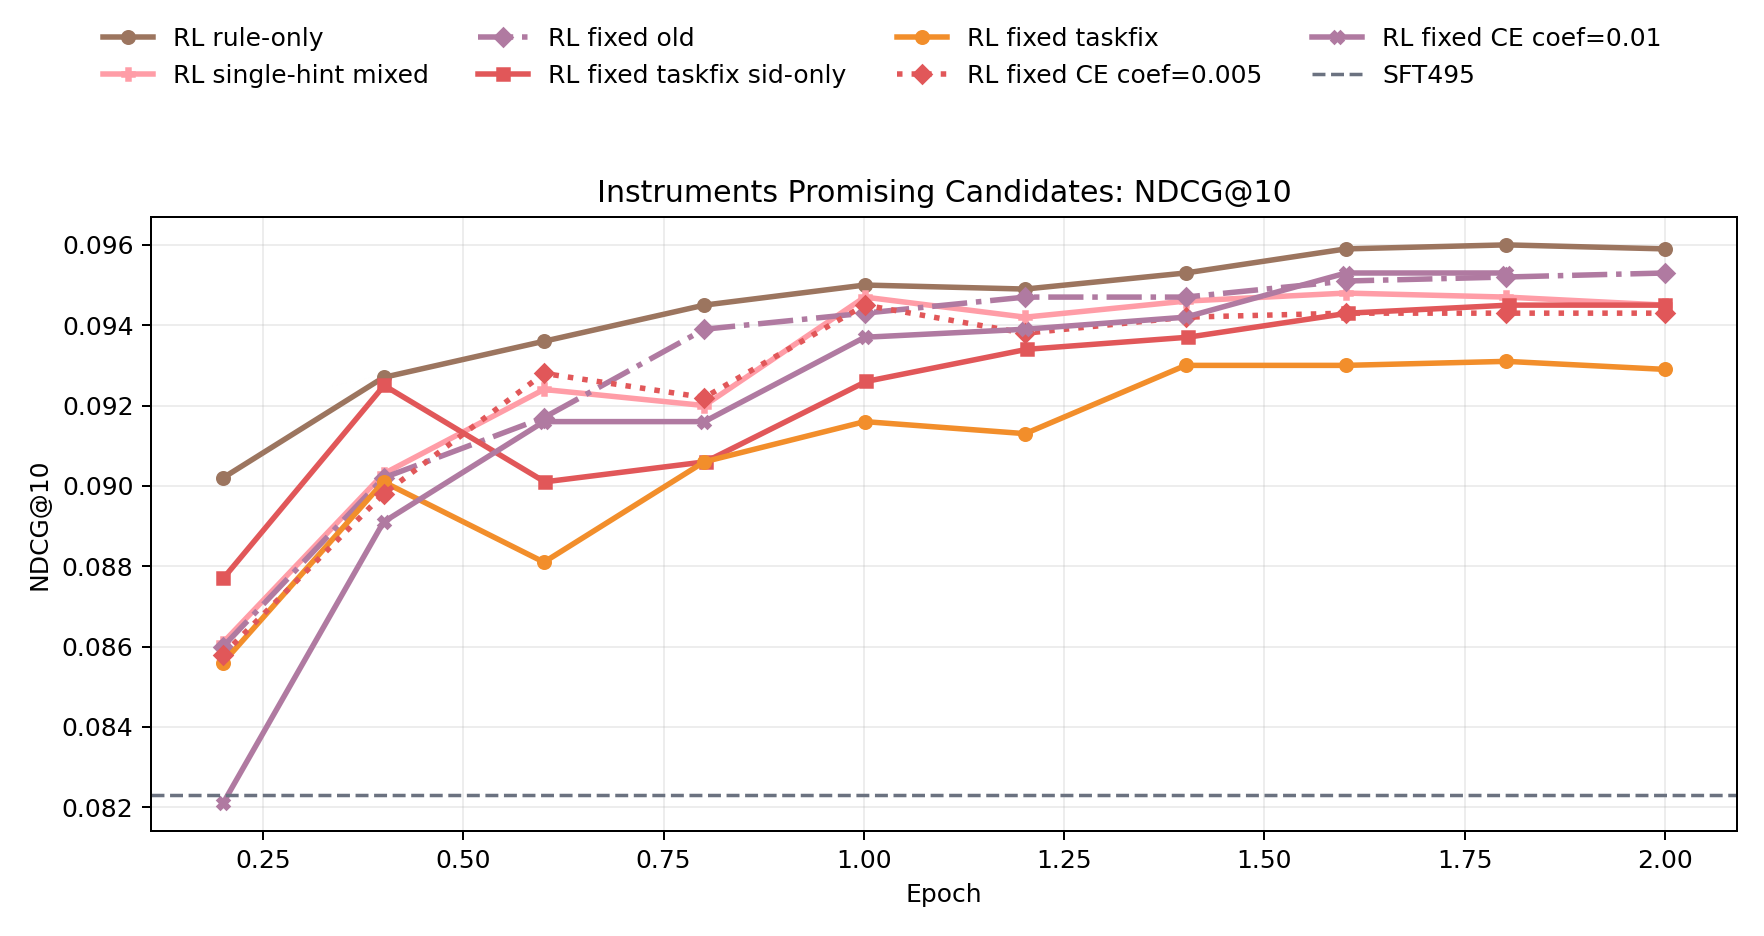
\includegraphics[width=0.96\textwidth]{promising_candidates_ndcg10.png}
\caption{Instruments promising candidates: NDCG@10。}
\end{figure}

\subsection{HR@10}

\begin{figure}[H]
\centering
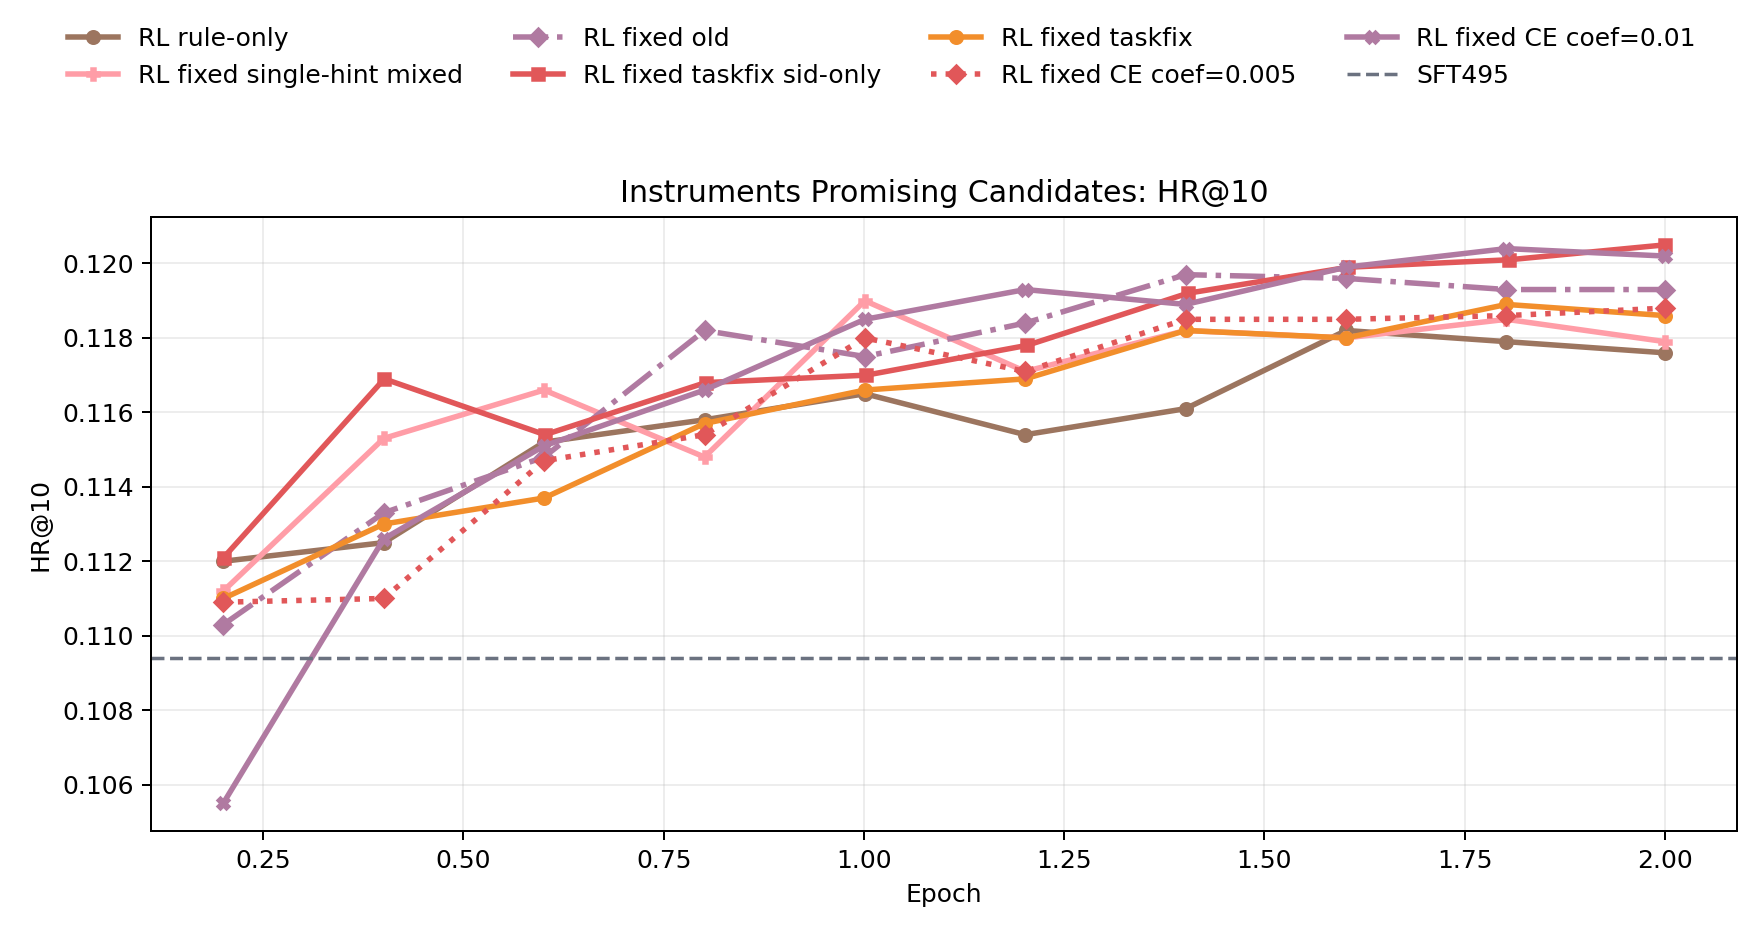
\includegraphics[width=0.96\textwidth]{promising_candidates_hr10.png}
\caption{Instruments promising candidates: HR@10。}
\end{figure}

\subsection{NDCG@50}

\begin{figure}[H]
\centering
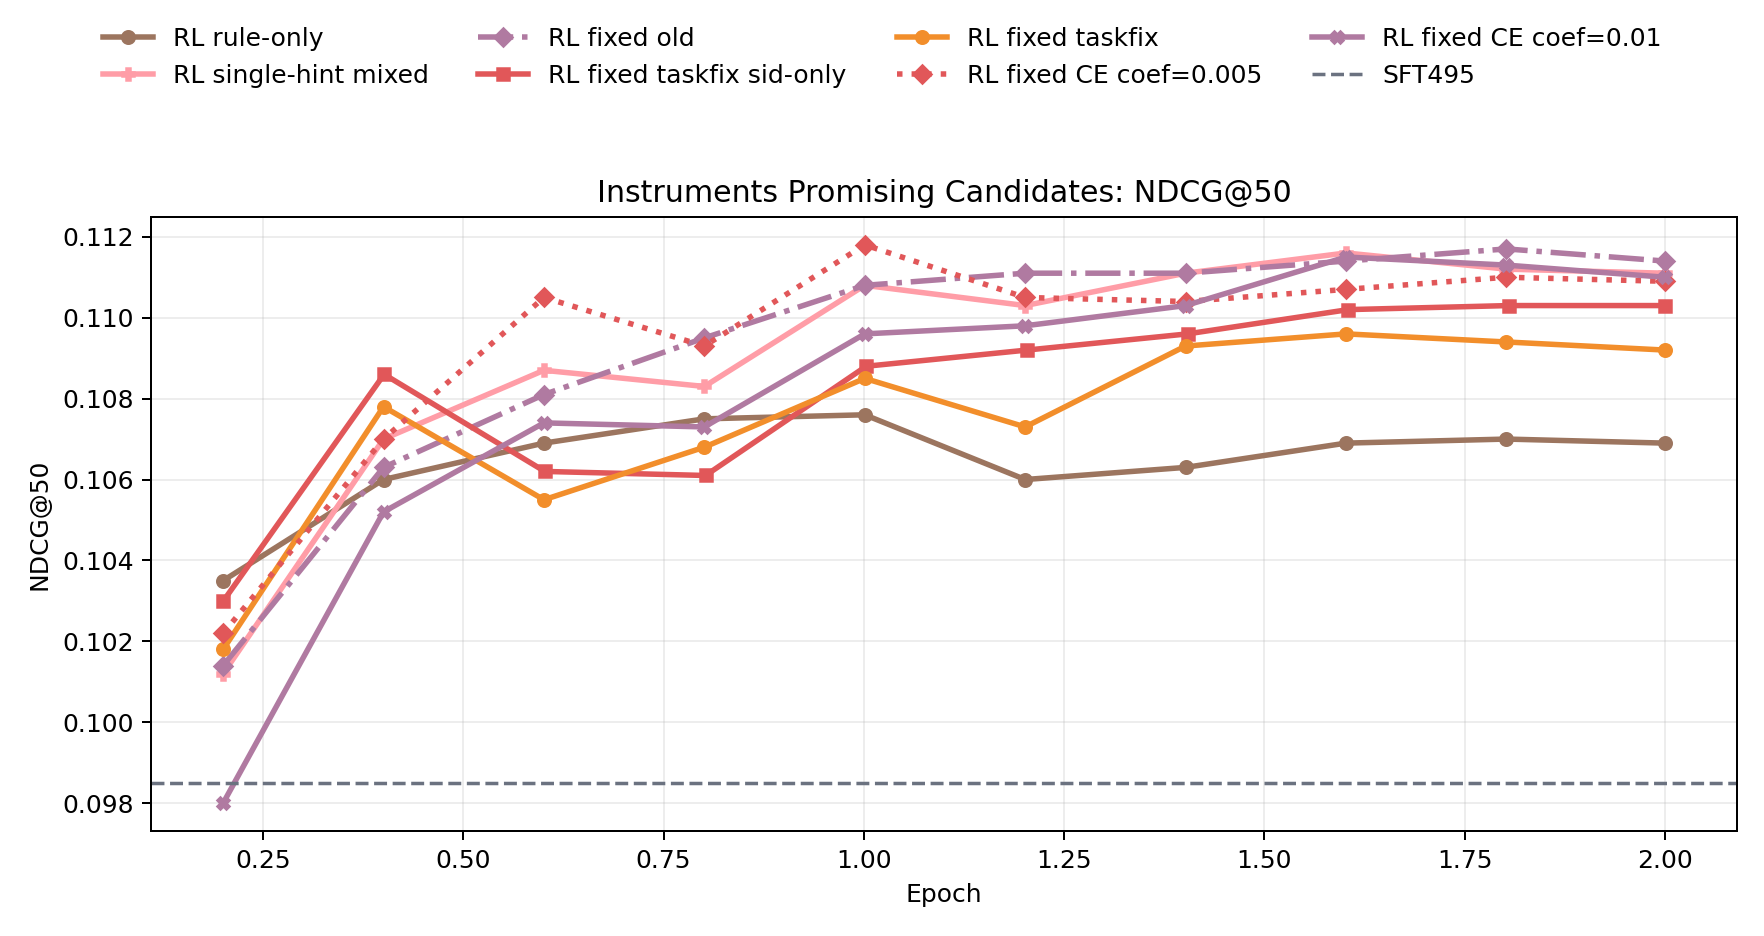
\includegraphics[width=0.96\textwidth]{promising_candidates_ndcg50.png}
\caption{Instruments promising candidates: NDCG@50。}
\end{figure}

\subsection{HR@50}

\begin{figure}[H]
\centering
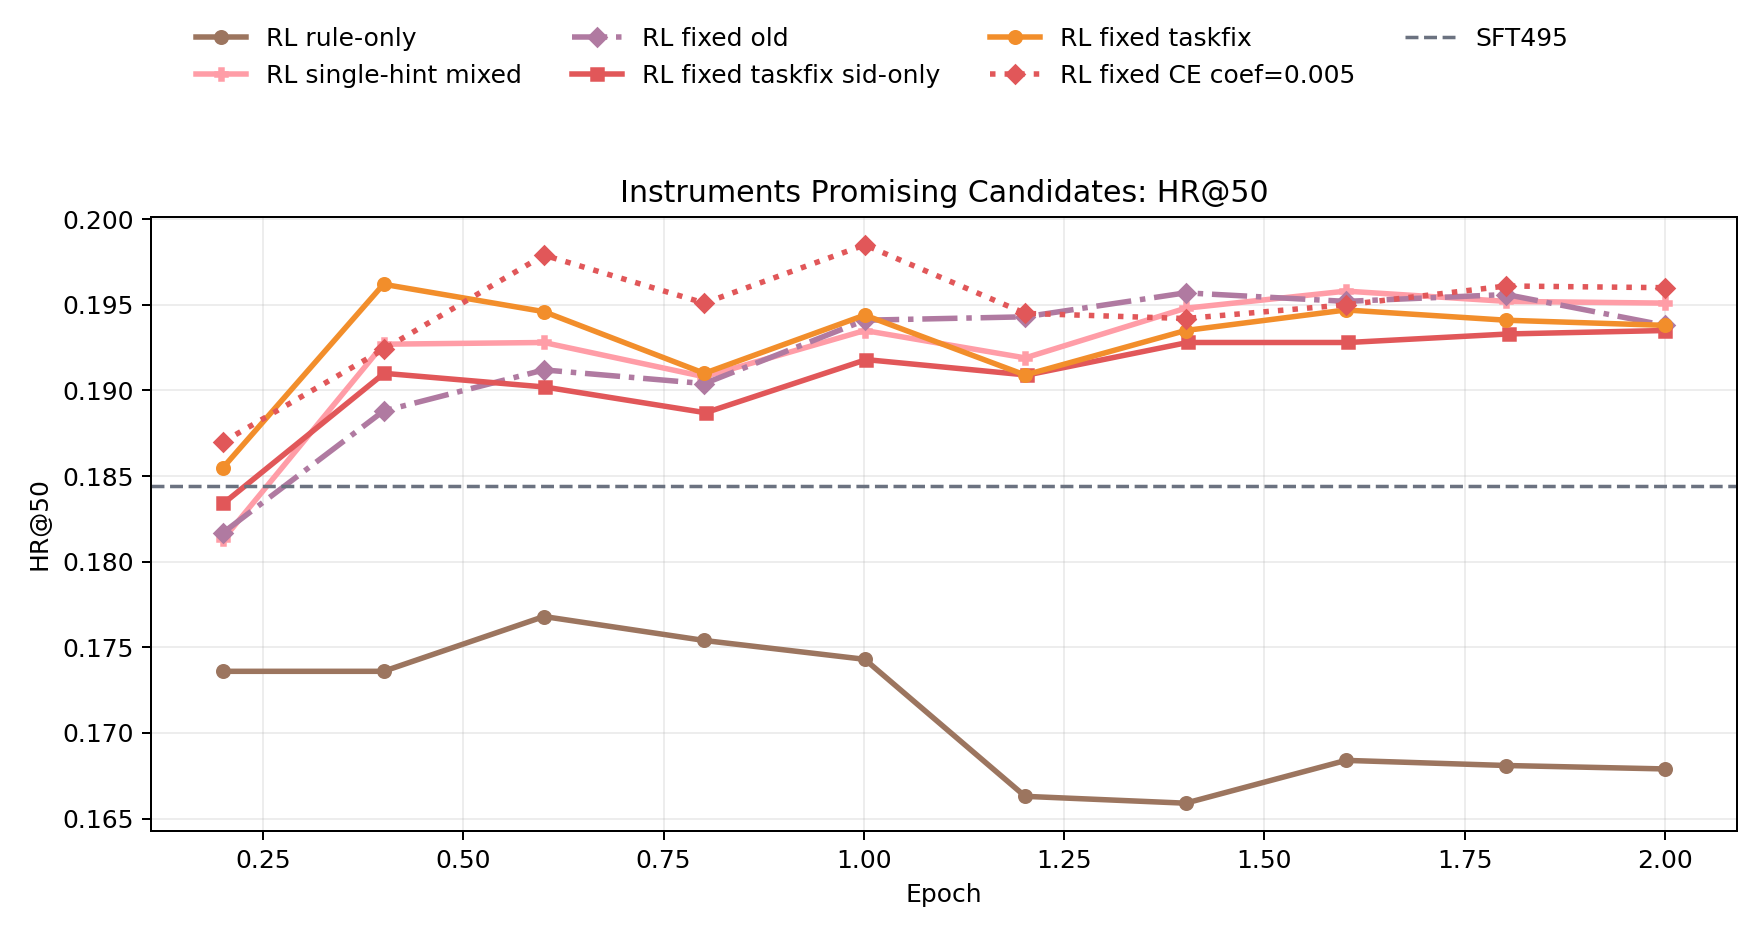
\includegraphics[width=0.96\textwidth]{promising_candidates_hr50.png}
\caption{Instruments promising candidates: HR@50。}
\end{figure}

\subsection{怎么读这一组图}

\begin{itemize}
\item 如果你只关心 headline top-10，\texttt{rule-only} 仍然是最靠上的线，但它在 \texttt{HR@50} 图里会立刻暴露 coverage 损失。
\item 如果你关心 clean fixed 主线，\texttt{fixed taskfix sid-only} 和 \texttt{fixed taskfix} 现在已经足够稳定，而且一个更偏 top-10，一个更偏 coverage。
\item 如果你关心新的最强候选，当前真正需要继续盯的不是单条 fixed，而是 \texttt{single-hint mixed} 和 \texttt{hintce-3}：
  前者更像完整长跑后的主候选，后者更像中段爆发出的高 coverage / 高 NDCG 新候选。
\item old \texttt{fixed mixed-single} 仍然有必要保留在图里，因为它提供了历史上界；但它只能当 historical reference，不能再当 clean 方法定义。
\end{itemize}

\section{Hint-Token SFT：去掉 RL 后的 Beam-Selected Hint Imitation}

\subsection{动机}

前面的 CE family 都是在 GRPO / DAPO 主损失旁边加一个 prompt-side CE：

\[
\mathcal{L}_{\text{total}}
= \mathcal{L}_{\text{RL}}
+ \lambda_{\text{CE}} \mathcal{L}_{\text{hint-CE}} .
\]

这次新设定把问题拆得更干净：不再让 reward、advantage、KL/reference model 或 completion-token policy gradient 参与更新，而是只训练模型在应该暴露 oracle hint 的位置上模仿真实 SID prefix token。换句话说，beam search rollout 只负责决定“这个样本至少需要多少个 hint token 才能解出来”，最终梯度只来自这些被选中的 hint token。

\subsection{代码入口}

{\footnotesize
\begin{itemize}
\item Trainer：\path{hint_sft_trainer.py}
\item fixed launcher：\path{hope/Qwen2_5-3B-Isntruct-qwen4B-4-256-MIMIGenRec-grec/Qwen2_5-3B-Isntruct-qwen4B-4-256-MIMIGenRec-grec-hint-token-sft-fixed.sh}
\item dynamic launcher：\path{hope/Qwen2_5-3B-Isntruct-qwen4B-4-256-MIMIGenRec-grec/Qwen2_5-3B-Isntruct-qwen4B-4-256-MIMIGenRec-grec-hint-token-sft-dynamic.sh}
\item 合成单测：\path{tests/test_hint_sft_trainer.py}
\end{itemize}
}

这两个 launcher 默认都跑 Instruments mixed 三任务，不再启用 \texttt{sid-hint-only} 或 task filter。也就是说，训练分布仍然覆盖 \texttt{task1\_sid\_sft}、\texttt{task4\_hisTitle2sid} 和 \texttt{task5\_title\_desc2sid}。

\subsection{Fixed 版本}

fixed 版本使用已有的 beam-hint 分析缓存作为 oracle depth 来源。启动脚本先调用
\path{analyze_rl_beam_hint.py}，从 \texttt{summary.json} / \texttt{details.json} 导出 fixed hint-depth map，然后把 map 注入训练集：

\[
d_i = \texttt{fixed\_hint\_depth\_map}(x_i).
\]

对每个训练样本，prompt 后拼接由 ground truth SID 构造出来的前 \(d_i\) 个 oracle token。若 \(d_i=0\)，该样本仍在 batch 中参与 padding 和 forward，但不会贡献 hint-token loss。若样本在离线 beam 分析里到最大深度仍未解出，默认使用 \texttt{fixed\_hint\_unsolved\_depth=3}。

\subsection{Dynamic 版本}

dynamic 版本把“需要多少 hint token”的选择放到训练时在线完成。对一个 batch，trainer 从 depth 0 开始构造 hinted prompt，用当前模型做 constrained beam rollout；如果某个样本任意 beam completion 和 ground truth SID 精确匹配，就选中当前 depth。没有命中的样本进入下一层 depth，直到 \texttt{dynamic\_hint\_max\_depth}。

需要强调的是：rollout completion 只是 selector，不进入监督标签。选中 depth 之后，真正反传的仍然只是 prompt 末尾的 oracle hint token CE。

\subsection{Loss 细节}

设拼好 hint 后的 token 序列为 \(z_i = [x_i, h_i]\)，其中 \(h_i\) 是 oracle hint prefix。代码构造 shift-label 位置上的 mask：

\[
m_{i,t} =
\begin{cases}
1, & z_{i,t+1} \in h_i,\\
0, & \text{otherwise}.
\end{cases}
\]

训练 loss 是 masked token mean：

\[
\mathcal{L}_{\text{hint-SFT}}
= \lambda_{\text{SFT}}
\frac{\sum_{i,t} m_{i,t}
\operatorname{CE}\left(p_\theta(\cdot \mid z_{i,\le t}), z_{i,t+1}\right)}
{\sum_{i,t} m_{i,t}} .
\]

实现上，DDP 下先 gather 全局 hint-token count，并把 denominator 按进程数缩放回每个 rank，这样各 rank 的梯度平均后等价于全局 token mean，而不是局部 token mean。若某个 batch 全局没有 hint token，则返回带梯度路径的 zero loss，避免反传时断图。

\subsection{和之前 CE / RL 的区别}

\begin{itemize}
\item 旧的 \texttt{fixed-hint-ce} 仍然先 rollout completion、算 reward、算 advantage，再用 RL loss 更新 completion policy；hint CE 只是旁路辅助项。
\item 新的 hint-token SFT 完全去掉 reward 计算、advantage 标准化、old/ref log-prob、KL penalty 和 completion-token RL 更新。
\item fixed 版本的 beam search 是离线 map 生成步骤；dynamic 版本的 beam search 是在线 depth selector。两者的共同点是 completion 本身都不作为 SFT 标签。
\item 旧 CE 里 \(\lambda_{\text{CE}}=0.005\) 是加在 RL 主 loss 旁边的相对倍率；新 SFT 没有 RL 主 loss，所以不能直接继续用 \texttt{lr=1e-5, coef=0.005} 当作同一个优化设定。
\end{itemize}

\subsection{学习率与 coef}

这个 setting 已经不是 RL loss 旁边的辅助 CE，而是一个纯 masked SFT objective。因此默认学习率不再按
\texttt{RL lr} 和 \texttt{hintce-3} 系数相乘，而是对齐 Instruments full SFT 配置
\path{examples/train_full/Instruments/instruments_rec_full_sft_3b_dsz0_qwen4b_4_256_grec.yaml}：

\[
\texttt{learning\_rate}=3.0\times10^{-4},
\qquad
\lambda_{\text{SFT}}=1.0.
\]

之前考虑过的 \(10^{-5}\times0.005=5\times10^{-8}\) 更适合解释“RL 主 loss 旁边的辅助 CE 有多重”，但放到纯 SFT 里会把 step size 压得过小。这里保留 \(\lambda_{\text{SFT}}=1.0\)，让 loss 本身就是标准 masked token mean；后续如果发现训练不稳，更自然的消融是直接扫 \texttt{learning\_rate}，例如 \texttt{1e-4} 或 \texttt{3e-5}，而不是重新引入一个很小的 loss coef。

\subsection{当前验证状态}

本地已经覆盖三个轻量检查：

\begin{itemize}
\item masked batch builder 只在 prompt suffix 的 oracle hint token 上打 CE mask。
\item fixed trainer 可以在合成数据上完整跑过一个 train step。
\item dynamic selector 可以选中最小成功 depth，并记录 selected-depth metric。
\end{itemize}

此外两个启动脚本都跑过 \texttt{--dry-run}，确认默认 5 epoch、\texttt{lr=3.0e-4}、\texttt{hint\_sft\_loss\_coef=1.0}，并且没有传入 task filter。真实结果跑完后，可以把 WandB / sidecar 指标接进现有 \texttt{docs/research/scripts/build\_instruments\_report\_figures.py} 画图流程。

\section{Games-grec 全流程摘要}

\subsection{为什么把 Games 放进附录}

当前这份研究稿主体仍然围绕 \texttt{Instruments-grec} 展开，因为那条线的变体更完整、家族内部对照也更多。相比之下，\texttt{Games-grec} 已经足够形成一条可复用的“单数据集 index $\rightarrow$ preprocess $\rightarrow$ SFT $\rightarrow$ RL”流水线，但更适合作为附录收录：

\begin{itemize}
\item 它已经能独立支撑一条完整的结果线，而不再只是实验脚手架。
\item 它当前最重要的价值，是验证 \texttt{fixed-hint > dynamic-hint > SFT} 这条大故事在另一个数据集上是否继续成立。
\item 它还没有像 Instruments 那样展开大量 family-internal ablation，因此不适合和正文混在同一层级叙述。
\end{itemize}

\subsection{Index 与下游数据}

\begin{table}[H]
\centering
\small
\setlength{\tabcolsep}{4pt}
\begin{tabular}{p{4.0cm} p{8.2cm}}
\toprule
项目 & 当前记录 \\
\midrule
Dataset & \texttt{Games} \\
Embedding model & \texttt{qwen3-embedding-4B} \\
Index config & \texttt{rq4(cb256-256-256-256)} \\
Final collision rate & \texttt{0.0075873} \\
Max conflict count & \texttt{5} \\
Layer utilization & 第 0 层 \texttt{47/256}；第 1/2/3 层 \texttt{256/256} \\
稳定 alias & \texttt{Games.index\_emb-qwen3-embedding-4B\_... \_dsGames.json} \\
\bottomrule
\end{tabular}
\caption{Games semantic index 的当前关键配置与结果。}
\end{table}

\begin{table}[H]
\centering
\small
\setlength{\tabcolsep}{4pt}
\begin{tabular}{p{3.2cm} c c}
\toprule
导出集合 & 规模 & 备注 \\
\midrule
SFT train & \texttt{520761} & 含 Task1/2/3 组合后的最终导出 \\
SFT valid & \texttt{42259} & 与 test 同量级 \\
SFT test & \texttt{42259} & 当前统一评测入口使用 \\
RL train & \texttt{280110} & 含 Task1/4/5 \\
RL valid & \texttt{42259} & 当前主要用于统一评测 \\
RL test & \texttt{42259} & 与 SFT test 对齐 \\
\bottomrule
\end{tabular}
\caption{Games-grec 下游数据导出规模。}
\end{table}

这里最重要的读法只有两点：

\begin{itemize}
\item 这个 \texttt{Games} index 的碰撞率已经低到足以进入下游 SFT/RL；后续重点不再是“能不能用”，而是“第 0 层 codebook 为什么利用率这么低”。
\item \texttt{Games\_grec} 已经不是只做了基础 preprocess 的半成品，而是完整支持统一 SFT / RL / evaluate 的正式变体。
\end{itemize}

\subsection{SFT checkpoint 选择}

\paragraph{对应入口}
{\footnotesize
\begin{itemize}
\item SFT YAML：\path{examples/train_full/Games/games_rec_full_sft_3b_dsz0_qwen4b_4_256_grec.yaml}
\item RL 默认初始化点：\texttt{Games-grec-sft-qwen4B-4-256-dsz0/checkpoint-896}
\item 本地出图脚本：\path{docs/research/scripts/build_games_report_figures.py}
\end{itemize}
}

\begin{table}[H]
\centering
\small
\setlength{\tabcolsep}{4pt}
\begin{tabular}{p{2.3cm} c c c c}
\toprule
Checkpoint & NDCG@10 & HR@10 & NDCG@50 & HR@50 \\
\midrule
\texttt{checkpoint-640} & 0.0426 & 0.0788 & 0.0680 & 0.1958 \\
\texttt{checkpoint-768} & 0.0433 & 0.0804 & 0.0691 & 0.1998 \\
\texttt{checkpoint-896} & 0.0430 & 0.0790 & 0.0687 & 0.1970 \\
\texttt{checkpoint-1024} & 0.0374 & 0.0692 & 0.0597 & 0.1729 \\
\bottomrule
\end{tabular}
\caption{Games SFT 后段 checkpoint 选择。}
\end{table}

\begin{figure}[H]
\centering
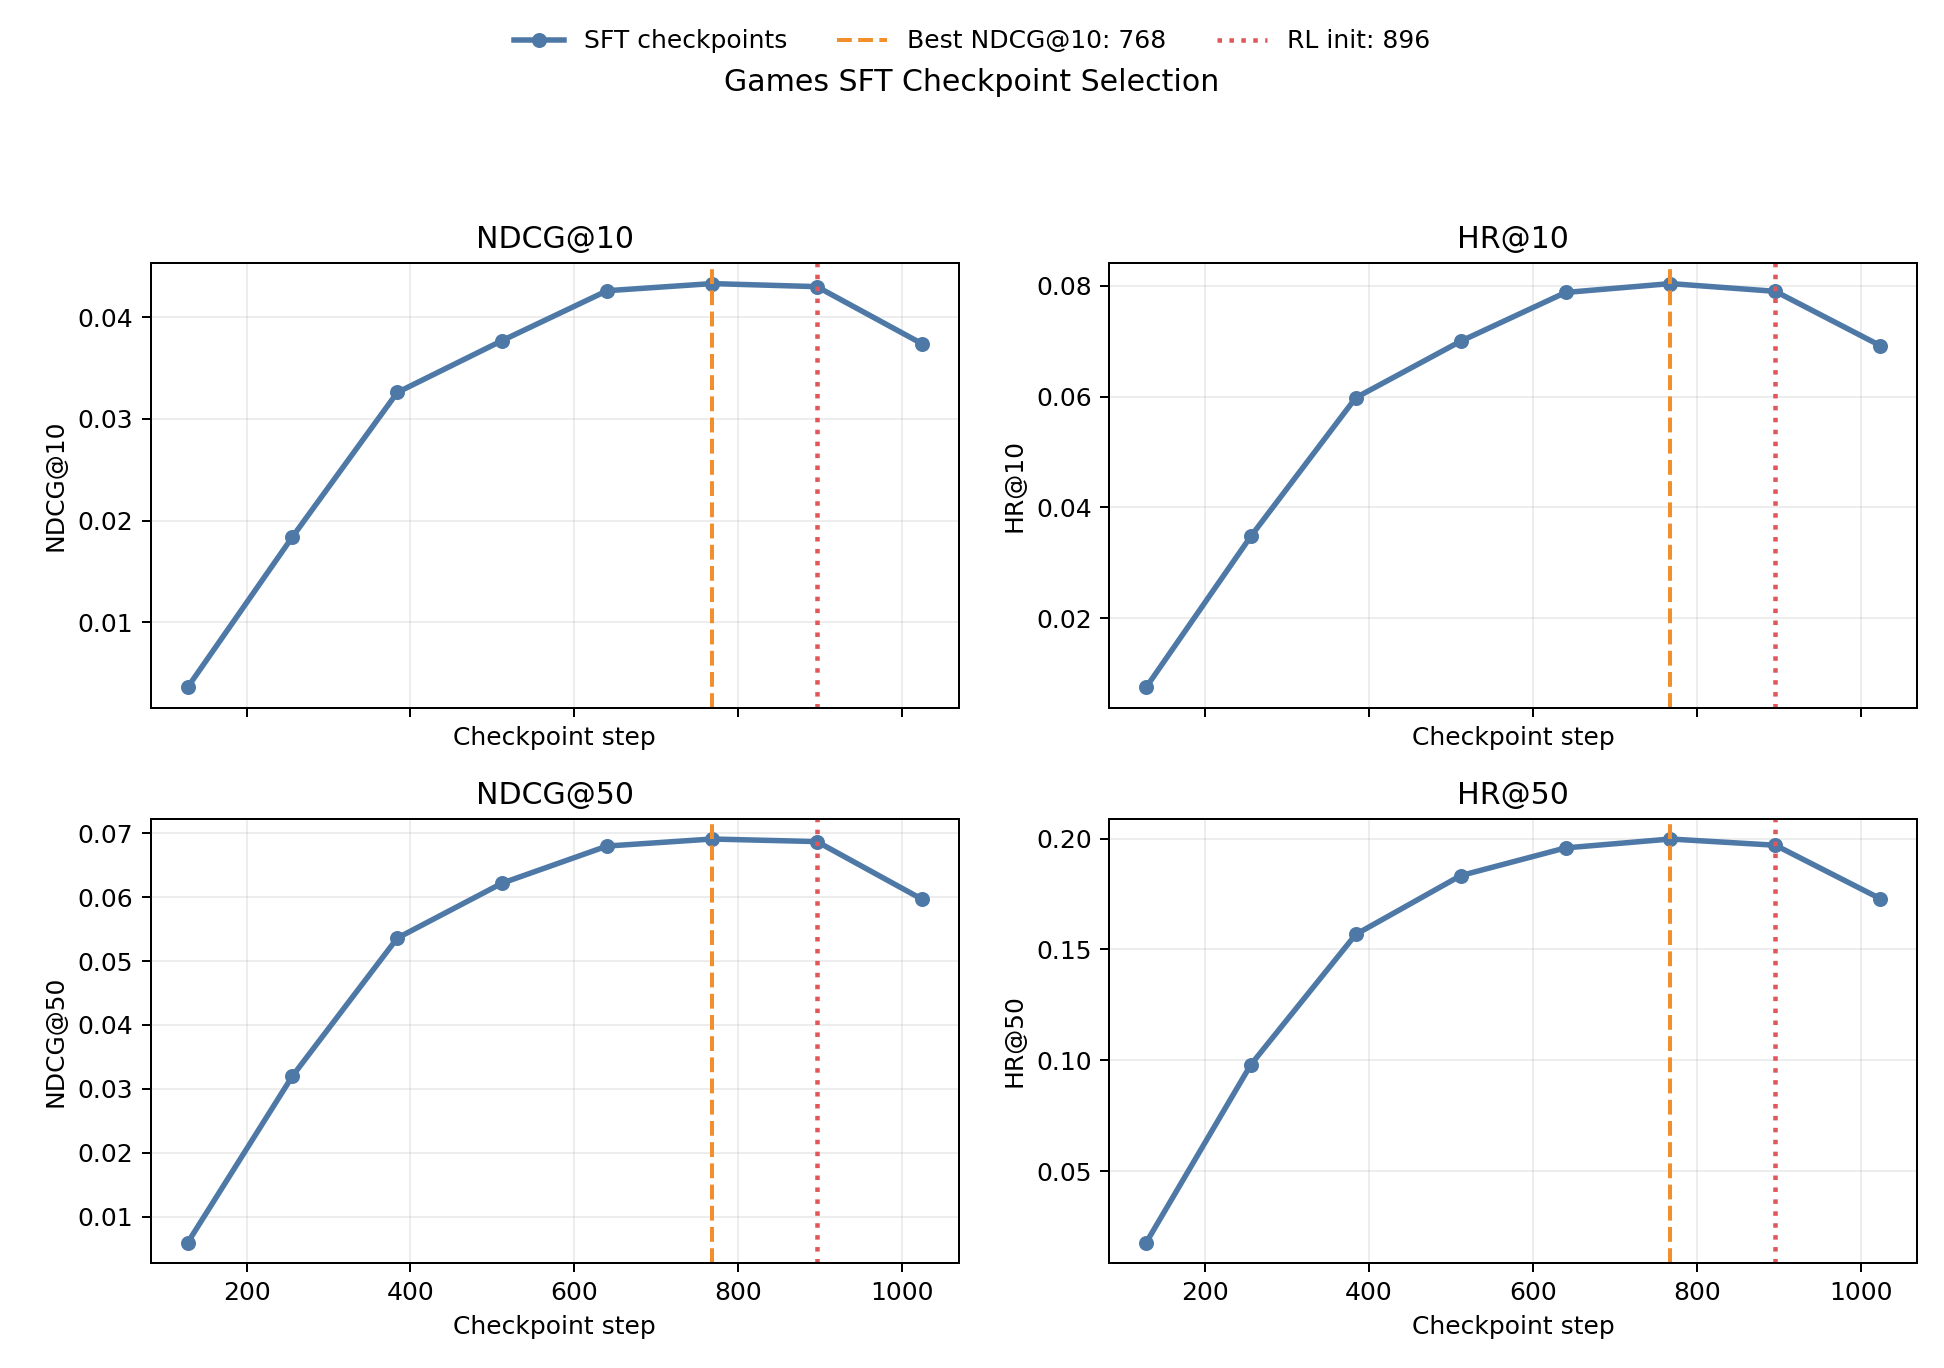
\includegraphics[width=0.96\textwidth]{games_sft_checkpoint_curves.png}
\caption{Games SFT checkpoint selection；虚线标出 best \texttt{NDCG@10} 的 \texttt{checkpoint-768}，点线标出 RL 默认初始化点 \texttt{checkpoint-896}。}
\end{figure}

这一段 SFT 的结论很清楚：

\begin{itemize}
\item 如果只按 best \texttt{NDCG@10} 选点，当前最强 SFT checkpoint 是 \texttt{768}。
\item 如果目的是继续接 RL，\texttt{896} 仍然是更稳妥的初始化点，因为它仍处在后段高性能平台里，但还没掉到 \texttt{1024} 那种明显回落区间。
\item 因此后文里的 Games RL，默认都把 \texttt{checkpoint-896} 当作统一起点。
\end{itemize}

\section{Games-grec RL 结果}

\subsection{对应 launcher}

{\footnotesize
\begin{itemize}
\item launcher 目录：\path{hope/Qwen2_5-3B-Isntruct-qwen4B-4-256-MIMIGenRec-Games-grec/}
\item rule-only：\path{Qwen2_5-3B-Isntruct-qwen4B-4-256-MIMIGenRec-Games-grec-rl-rule-only.sh}
\item dynamic-hint：\path{Qwen2_5-3B-Isntruct-qwen4B-4-256-MIMIGenRec-Games-grec-rl-rule-only-dynamic-hint.sh}
\item fixed-hint：\path{Qwen2_5-3B-Isntruct-qwen4B-4-256-MIMIGenRec-Games-grec-rl-rule-only-fixed-hint.sh}
\item 本地出图脚本：\path{docs/research/scripts/build_games_report_figures.py}
\end{itemize}
}

\subsection{最好点与 coverage 峰值}

\begin{table}[H]
\centering
\small
\setlength{\tabcolsep}{4pt}
\begin{tabular}{p{2.7cm} p{2.4cm} c c c c}
\toprule
Variant & Best ckpt & NDCG@10 & HR@10 & NDCG@50 & HR@50 \\
\midrule
SFT best & \texttt{checkpoint-768} & 0.0433 & 0.0804 & 0.0691 & 0.1998 \\
RL rule-only & \texttt{checkpoint-8752} & 0.0467 & 0.0825 & 0.0683 & 0.1815 \\
RL dynamic-hint & \texttt{checkpoint-4380} & 0.0464 & 0.0823 & 0.0716 & 0.1980 \\
RL fixed-hint & \texttt{checkpoint-8752} & 0.0480 & 0.0857 & 0.0723 & 0.1972 \\
\bottomrule
\end{tabular}
\caption{Games-grec 上 SFT 与三条 RL 主线的最好点。}
\end{table}

\begin{table}[H]
\centering
\small
\setlength{\tabcolsep}{4pt}
\begin{tabular}{p{2.7cm} p{2.4cm} c c}
\toprule
Variant & Peak \texttt{HR@50} ckpt & Peak \texttt{HR@50} & 同点 \texttt{NDCG@10} \\
\midrule
RL rule-only & \texttt{checkpoint-4380} & 0.1851 & 0.0463 \\
RL dynamic-hint & \texttt{checkpoint-3504} & 0.1981 & 0.0461 \\
RL fixed-hint & \texttt{checkpoint-3504} & 0.2024 & 0.0478 \\
\bottomrule
\end{tabular}
\caption{Games RL 三条线的 coverage 峰值。}
\end{table}

从这两张表可以直接读出当前阶段性排序：

\begin{itemize}
\item 按 best \texttt{NDCG@10} 看，Games 当前已经形成 $\texttt{fixed-hint} > \texttt{rule-only} \gtrsim \texttt{dynamic-hint} > \texttt{SFT}$。
\item plain \texttt{rule-only} 继续体现出和 Instruments 相同的模式：top-10 变强，但 \texttt{HR@50} 掉得最明显。
\item \texttt{dynamic-hint} 仍然是很有竞争力的第二梯队；它在自己 best top-10 点上的 \texttt{HR@50} 仍略高于 late-stage \texttt{fixed-hint}。
\item 如果改按 coverage 峰值而不是 best \texttt{NDCG@10} checkpoint 读，\texttt{fixed-hint} 的 \texttt{checkpoint-3504 / HR@50=0.2024} 仍然是全场最强点。
\end{itemize}

\subsection{RL 曲线图}

\begin{figure}[H]
\centering
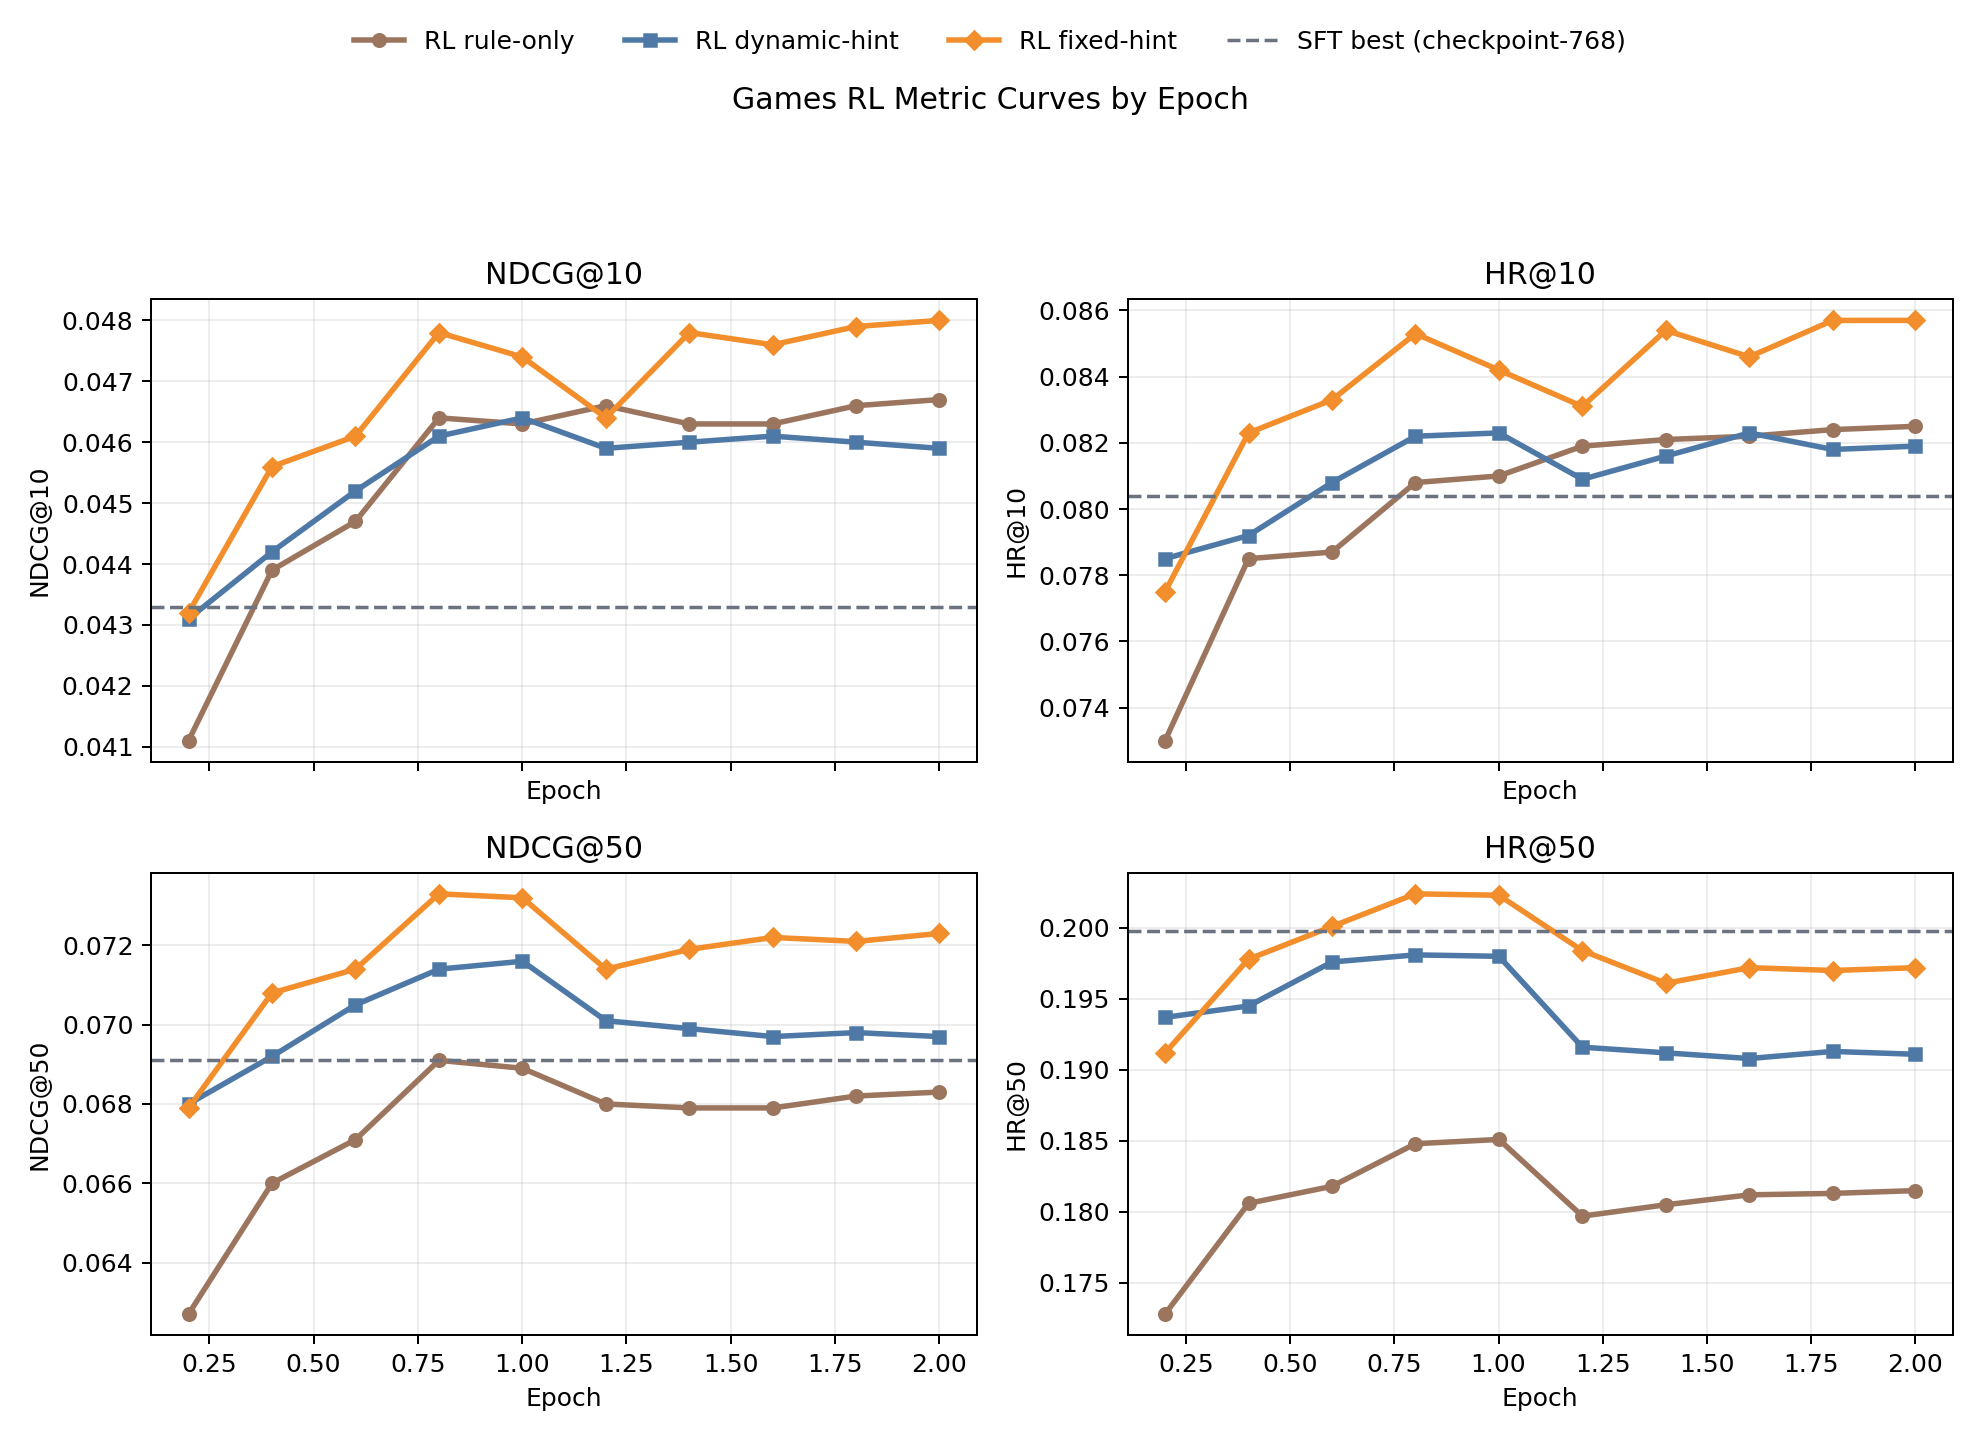
\includegraphics[width=0.96\textwidth]{games_rl_epoch_curves.png}
\caption{Games RL metric curves；灰虚线是 SFT best \texttt{checkpoint-768} 的水平参考线。}
\end{figure}

这张图更适合用来解释“最佳点为什么不在同一时刻”：

\begin{itemize}
\item \texttt{rule-only} 在 \texttt{NDCG@10} 上还能慢慢涨到尾点，但 \texttt{HR@50} 很早就进入平台区，后面也没有明显恢复。
\item \texttt{dynamic-hint} 的最佳窗口集中在 \texttt{epoch}$\approx$\texttt{1.0} 左右；同步到完整 \texttt{2 epoch} 之后，它并没有继续把 top-10 往上抬。
\item \texttt{fixed-hint} 呈现很典型的“两段式最优”：中前段先拿到全场最强 coverage，训练末端再把 \texttt{NDCG@10 / HR@10} 推到新的最高点。
\end{itemize}

\subsection{最好点 trade-off}

\begin{figure}[H]
\centering
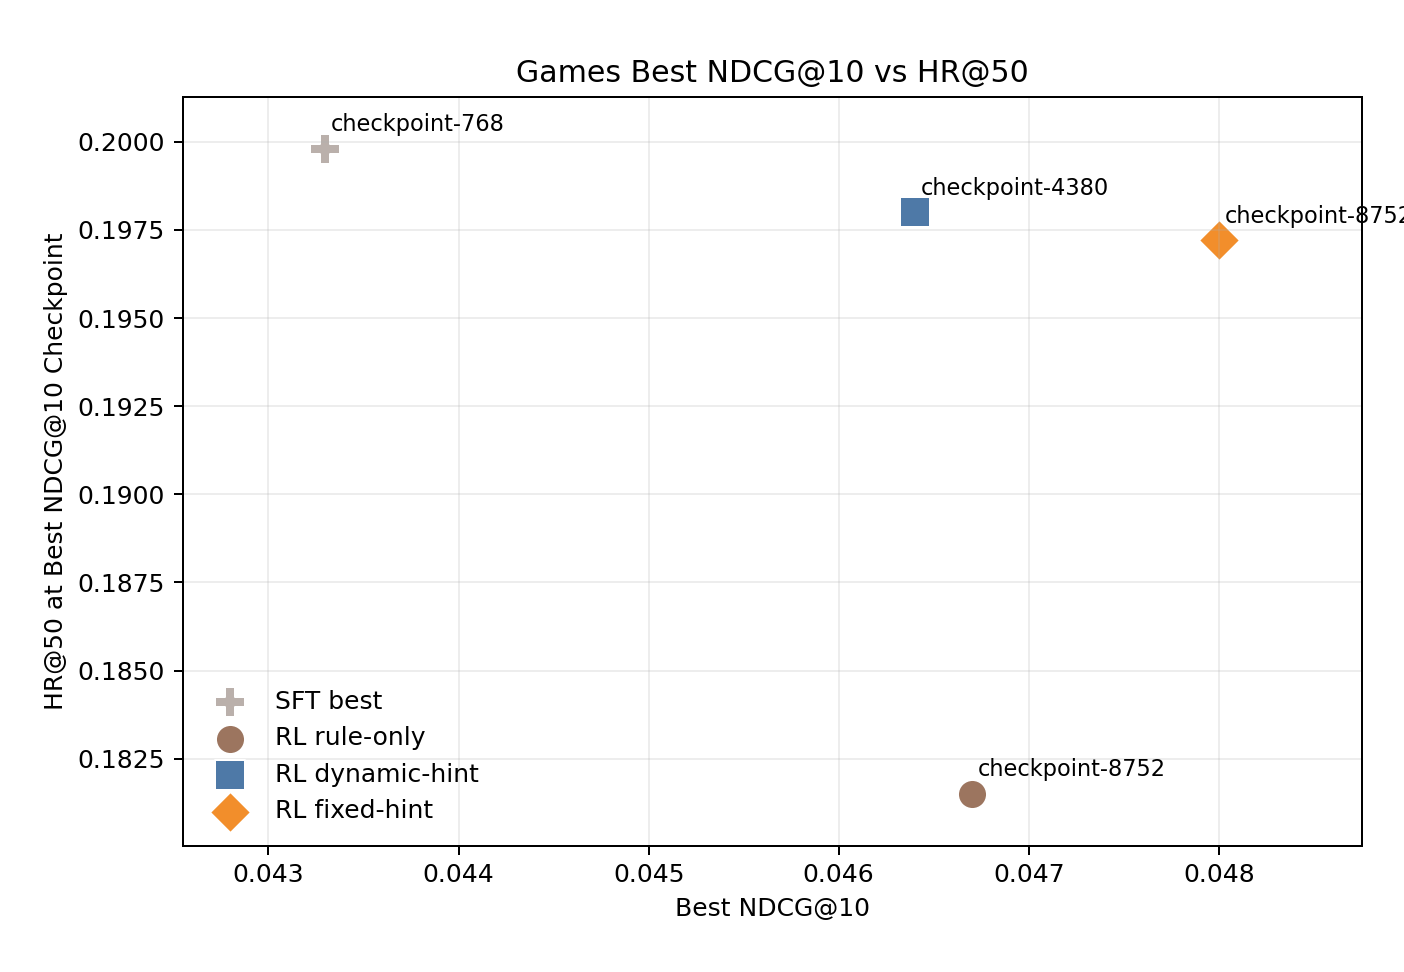
\includegraphics[width=0.80\textwidth]{games_best_ndcg10_vs_hr50_scatter.png}
\caption{Games best \texttt{NDCG@10} vs \texttt{HR@50} scatter。}
\end{figure}

如果把每条线都压成一个 best 点，这张散点图最值得记住三件事：

\begin{itemize}
\item 最靠右的是 \texttt{fixed-hint}，说明它当前已经拿到了 Games 上最强的 top-10 点。
\item \texttt{dynamic-hint} 虽然右移不如 \texttt{fixed-hint}，但它在自己 best 点上的 \texttt{HR@50} 仍然处在高位，因此它不是失败 run，而是“coverage 更稳、top-10 略弱”的第二梯队。
\item \texttt{rule-only} 则明显更靠下，说明它在 Games 上也复现了“top-10 强、coverage 弱”的交换。
\end{itemize}

\subsection{当前读法}

把 Games 这条线纳入附录之后，当前最稳妥的总结是：

\begin{enumerate}
\item \texttt{Games-grec} 已经不再只是辅助数据集，而是完成了一条可复用的单数据集全流程。
\item 在第二个数据集上，\texttt{fixed-hint} 仍然是当前最平衡的主线，说明 Instruments 上的主故事并不是单点偶然。
\item \texttt{dynamic-hint} 仍然有明确价值，但它现在更像“覆盖率更稳的次优 family”，而不是已经改写主线排序的方案。
\item 如果后面继续扩 Games，最值得补的是 task-level readout，以及 \texttt{fixed-hint} 的 best-top10 点和 best-coverage 点之间到底该如何汇报。
\end{enumerate}


\end{document}
